\clearpage

\section {Systematic effects in the prediction of the single $\mu$-like ring event energy spectrum}
\label{sec:systematics}

%....................................................................................................................
%....................................................................................................................

\subsection {Input systematic parameters}
\label{sec:systematics:inputs}

This analysis considers 45 systematic parameters which can be grouped into 5 categories:

\begin{enumerate}

\item 
{\bf SuperK energy scale} (1 parameter).\\
The systematic parameter $f_{E; r}^{SK}$ is included to control the energy scale.
Its uncertainty is estimated to be 2.4\% \cite{SuperkEScale2013}.
The effect of the uncertainty in the reconstructed energy scale is calculated by scaling the bin edges of
the MC templates and, assuming uniform distribution of events within the bins, calculating the number
of events gained from / lost to neighbouring bins. 
The effect of the energy scale uncertainty is propagated to all MC templates as shown in Tab.\ \ref{tab:apply_syst_to_templates}.\\

\item 
{\bf SuperK efficiencies \& effects of intranuclear and secondary re-interactions} (6 parameters).\\
There are uncertainties in the efficiencies of the fiducial volume and reduction chain, 
and the OD, ring-counting, PID, momentum and decay-electron cuts.
These uncertainties have been evaluated by comparing 1412 days of SK-IV atmospheric data
with atmospheric neutrino Monte Carlo.
Ring counting errors are evaluated using $\nu_\mu$ CCQE, $\nu_\mu$ CCnQE, NC, and $\nu_e$ CC-enriched control samples.
The NC PID error is evaluated using a NC-enriched control sample, which
does not use PID information.
Each Monte Carlo control sample is fitted to the data using the efficiency as a fit parameter, and the uncertainties in the 
efficiencies are estimated by adding the covariance matrix containing the differences between the best-fit and nominal efficiencies to 
the covariance matrix containing the statistical errors in the fitted efficiencies \cite{SuperkErrors2013}.

Intranuclear final-state interactions (FSI) have significant effects in the T2K energy range and
result in event topologies, for scattering from nuclear targets, which are drastically different from 
those created in neutrino scattering from free nucleons.
Uncertainties due to FSI were estimated by simultaneously varying the NEUT parameters that scale the interaction probabilities for quasi-elastic 
scattering, absorption, charge exchange and pion production using the method described in Sec.\ 2 in \cite{NIWGErr}. The NIWG group produced 16 
parameter sets that span the 1$\sigma$ surface in the parameter space; this was done by varying the NEUT parameters when running the pion scattering 
simulations, and comparing the results with external pion-carbon scattering data. These 16 parameter sets are shown in Tab.\ 2 in \cite{NIWGErr}. 
Uncertainties due to secondary pion interactions (SI) were also evaluated. The NIWG group adapted the NEUT nuclear cascade model to simulate SI in the 
SuperK detector simulation (SKDETSIM) and to allow variations in the interaction probabilities. Details of this are given in \cite{SI}. 
Since the same model is used for FSI and SI, it is possible to evaluate the uncertainties in both FSI and SI simultaneously. This was done by 
reweighting a single $\mu$-like ring selected SK MC with the 16 FSI parameter sets using T2KReweight. The reweighting method for FSI is described 
in Sec. 8 in \cite{NEUTnuclear}. Variations in the SI interaction probabilities were included for each FSI parameter set.  Subsequently a covariance 
matrix was calculated using equation 1 in \cite{NIWGErr}; the quantity p in that equation is the average event weight for a FSI parameter set, and 
the sum is over the parameter sets.

In this analysis, we consider the SuperK detector efficiency and FSI/SI systematics together, and add their covariance matrices linearly. Each of 
these covariance matrices has six correlated parameters, corresponding to different modes and reconstructed energy bins, as shown in Tab.\ \ref{tab:input_uncertainties}.
These efficiency/FSI/SI systematics are applied to the MC templates as shown in Tab.\ \ref{tab:apply_syst_to_templates}.\\

\item 
{\bf Correlated flux and cross-section (BANFF) parameters} (23 parameters).\\
The postfit uncertainties of all BANFF flux and cross-section parameters and their correlations are taken into account.
For the disappearance analysis, we use a version of the BANFF fit which considers
only the $\nu_\mu$ and $\bar{\nu}_{\mu}$ flux parameters. The effect of the $\nu_{e}$ and $\bar{\nu}_{e}$ 
flux parameter uncertainties was studied and it was found to be negligible \cite{OurRun123DisappAnalysis3Flavour}.
Only those cross-section parameters that are expected to have some cancellation between the ND280 and SuperK are included in the BANFF fit.
%The other cross-section parameters included in this analysis are taken to be uncorrelated with the flux parameters
%and to have no cancellation between the near and far detectors. These uncorrelated cross-section parameters are discussed below.
A list of the BANFF parameters, their best-fit values and their prefit and postfit errors is given in Tab.\ \ref{tab:input_uncertainties}.

The BANFF parameters are applied to the MC templates as specified in Tab.\ \ref{tab:apply_syst_to_templates}.
All but two of the BANFF cross-section parameters are simple normalization factors.
The parameters $f_{16; t, r}^{banff}$ and $f_{17; t, r}^{banff}$ are
the axial masses that are parameters in the models of neutrino CC quasi-elastic ($M_{A}^{QE}$) 
and resonance-production ($M_{A}^{RES}$) interactions respectively;
these have a more complicated, often non-linear, dependence on true and reconstructed neutrino energy.
Event reweighting methods were used to obtain the fractional changes of the number of events, 
in bins of true and reconstructed neutrino energy, for a range of values (-3.0$\sigma$, -2.5$\sigma$, -2.0$\sigma$, ..., +3.0$\sigma$)
in the $f_{16; t, r}^{banff}$ and $f_{17; t, r}^{banff}$ parameters.
In our p.d.f. calculation, cubic splines\footnote{
  In this analysis, the cubic splines are computed for each non-linear systematic and for each MC template,
  in bins of reconstructed and true energy. To produce these splines, we use the SK13a SuperK MC, the 11bv3.2 flux weights and 
  the following oscillation parameters: $\sin^{2}(2\theta_{23})$ = 1.0, $\sin^{2}(2\theta_{13})$ = 0.098, $\sin^{2}(2\theta_{12})$ = 
  0.8495, $|\Delta m^{2}_{32}|$ = 2.44$\times$10$^{-3}$ eV$^{2}$/c$^{4}$, $\Delta m^{2}_{21}$ = 7.5$\times$10$^{-5}$ eV$^{2}$/c$^{4}$, 
  $\delta_{CP}$ = 0 and the normal mass hierarchy. For all splines, we use 41 bins in reconstructed energy:
  1 bin from 0-0.3 GeV, 14 50-MeV bins from 0.3-1.0 GeV, 20 100-MeV bins from 1.0-3.0 GeV, 2 500-MeV bins from 3.0-4.0 GeV
  1 bin from 4.0-5.0 GeV, 1 bin from 5.0-7.0 GeV, 1 bin from 7.0-10.0 GeV and 1 bin from 10.0-30.0 GeV.
  The $\nu_{\mu}$, $\bar{\nu}_{\mu}$ and oscillated $\nu_{e}$ samples have 11 bins in true energy:
  1 bin from 0-0.4 GeV, 3 100-MeV bins from 0.4-0.7 GeV, 1 bin from 0.7-1.0 GeV, 1 bin from 1.0-1.5 GeV, 2 1-GeV bins from 1.5-3.5 GeV,
  1 bin from 3.5-5.0 GeV, 1 bin from 5.0-7.0 GeV and 1 bin from 7.0-30.0 GeV.
  The $\nu_{e}$ and oscillated $\nu_\mu$ samples have 7 bins in true energy:
  1 bin from 0-0.05 GeV, 1 bin from 0.5-0.7 GeV, 1 bin from 0.7-0.8 GeV,
  1 bin from 0.8-1.5 GeV, 1 bin from 1.5-2.5 GeV, 1 bin from 2.5-4.0 GeV and 1 bin from 4.0-30.0 GeV.
  Finally, the $\bar{\nu}_{e}$ sample have 2 bins in true energy:
  1 bin from 0-2.5 GeV and 1 bin from 2.5-30.0 GeV.\\
  The binning of the cubic splines was studied, and the results were presented in Appendix I of \cite{OurRun123DisappAnalysis3Flavour}.
  The spline spectra produced using the cubic splines are very similar to those produced using the CPU-intensive event-by-event reweighting,
  especially for the dominant components of the spectra. 
} 
are used to interpolate between these event weights 
to obtain the fractional change for any value of these systematic parameters in the (-3.0$\sigma$, +3.0$\sigma$) range.\\

\item 
{\bf Uncorrelated cross-section parameters}(11 parameters).\\
In addition to the BANFF cross-section systematics,
another 11 cross-section systematics are taken into account; these additional systematics are considered to be uncorrelated 
between themselves and to have no cancellation between the near and far detectors \cite{NIWGErr} \cite{MoreNIWGErr113} \cite{NIWGNuBarErr}.

Three of these additional systematics relate to the initial-state nuclear environment modelling for CCQE.
Neutrino Monte Carlo generators typically use Relativistic Fermi Gas (RFG) models,
with or without extensions to take nucleon-nucleon correlation into account, 
and with some, often simplistic, prescription for the treatment of off-shell kinematics.
The RFG model implementation depends on two parameters, the Fermi momentum level (225 MeV for $^{16}O$)
and the nucleon binding energy (27 MeV for $^{16}O$), which are extracted from quasi-elastic electron scattering data.
The systematic parameter $f_{pF; t, r}$ takes into account the effect of a 30 MeV 1$\sigma$ uncertainty in the Fermi momentum level
for $^{16}O$, while the parameter $f_{bindE; t, r}$ takes into account the effect of a 9 MeV 1$\sigma$ uncertainty in the nucleon 
binding energy for for $^{16}O$.
The implementation details of the nuclear model can have a significant effect and, therefore,
the effect of switching between two such models was also included as a systematic uncertainty.
This analysis considers the effect of switching between the RFG model and a better-motivated 
Spectral Function (SF) model. The latter does not assume a fixed binding energy and includes the 
correlations between nucleon momentum and binding energy. The systematic parameter $f_{SF; t, r}$ 
includes the effect of switching between the two models.

Simple, energy-independent, generator-level uncertainties are considered for the CC coherent, NC, $\nu_e$ CC
and $\bar{\nu}$ CC cross sections, as the effect of these processes in the single $\mu$-like ring sample is small.
This analysis uses a 100\% uncertainty for the CC coherent cross-section, 
a 30\% uncertainty for both the NC1$\pi^\pm$ and NC ``other'' (all but single $\pi^\pm$) cross section,
a 3\% uncertainty on the $\nu_e$ / $\nu_\mu$ CC cross-section ratio and 
a 20\% uncertainty on the $\bar{\nu}$ / $\nu$ CC cross-section ratio.
The effect of the variation of the above cross sections is included in the analysis
through the systematic parameters $f_{CCcoh; t}$, $f_{NC1\pi^\pm; t}$, $f_{NCoth; t}$,
$f_{CC\nu_e; t}$ and $f_{CC\bar{\nu}; t}$ respectively.

The treatment of $\Delta$ resonances in the nuclear environment has been controversial in the neutrino
Monte Carlo generator community. Certain models include a ~20\%-level of $\pi$-less $\Delta$ decays in order
to include the effect of $\Delta+N \rightarrow N+N$ scattering, in which the $\Delta$ interacts before it can decay. 
In contrast, other models include no $\pi$-less 
$\Delta$ decays on the basis that this would amount to double counting since, whatever the size of the effect, 
it is already included in hadron-nucleus scattering data to which the intranuclear cascade Monte Carlos are tuned.
This analysis uses NEUT, in which 20\% of $\Delta$s have a $\pi$-less decay by default, and takes the uncertainty in this 
branching fraction to be 100\%. 
The systematic parameter $f_{\pi-less\Delta; t, r}$ includes the effect of varying the fraction of $\pi$-less $\Delta$ 
decays to the corresponding MC templates.

The $f_{CCothShape;t,r}$ systematic parameterizes the uncertainty in CC multi-pion, CC deep inelastic scattering and CC $\eta$, 
K and photon production. From MINOS data, this is known to be $\approx$10\% at 4 GeV. Using this as a reference point, 
the uncertainty is estimated as 0.4/E$_{\nu}$, where E$_{\nu}$ is in GeV. It might appear that this error could diverge at 
low energy, but this does not happen since the threshold is $\approx$0.6 GeV and there are very 
few interactions below 1 GeV. 

The $f_{Wshape;t,r}$ parameter modifies the shape of the initial pion momentum distribution (before final-state interactions) 
by changing the distribution of the pion/nucleon invariant mass while keeping the total cross section constant. As the 
W shape parameter decreases, the pion momentum shifts to lower values, and this increases the probability of pion 
absorption in a final-state interaction. If such an absorption occurs, the event is migrated from CC1$\pi$ (its 
true initial state) and appears to be CCQE.

The effect of the $f_{CCcoh; t}$, $f_{NC1\pi^\pm; t}$, $f_{NCoth; t}$, $f_{CC\nu_e; t}$ and $f_{CC\bar{\nu}; t}$ 
systematic parameters is a simple normalisation change for the corresponding MC templates and thus easily implemented.
Systematic parameters $f_{pF; t, r}$, $f_{SF; t, r}$, $f_{bindE; t, r}$, $f_{\pi-less\Delta; t, r}$, $f_{CCothShape; t, r}$ 
and $f_{Wshape; t, r}$  have a complicated, often non-linear, dependence on true and reconstructed energy.
These are treated in a similar way to the BANFF parameters $f_{16; t, r}^{banff}$ and $f_{17; t, r}^{banff}$.
Event reweighting methods were used to obtain the fractional changes of the number of events, 
in bins of true and reconstructed neutrino energy, for a range of values (-3.0$\sigma$, -2.5$\sigma$, -2.0$\sigma$, ..., +3.0$\sigma$)
of the systematic parameters. Again cross-section splines with polynomials of order 3 were used to interpolate between these event 
weights to obtain the fractional change for any
value of these systematic parameters in the (-3.0$\sigma$, +3.0$\sigma$) range.

Some of these systematics are special cases:
{
\begin{itemize}
\item 
  $f_{SF; t, r}$ is discrete; it can be either spectral function off (RFG) or spectral function on (SF). 
  Splines are generated with SF off as nominal (0), and SF on as +1$\sigma$.
  This parameter is restricted to the range between 0 and +1$\sigma$, and linear interpolation is made between the weights 
  for nominal and +1$\sigma$.
\item 
  For $f_{Wshape; t, r}$ only $\pm$1$\sigma$ errors are evaluated using event reweighting. 
  Weights for positive tweaks are interpolated or extrapolated from the nominal and +1$\sigma$ weights, and weights for negative 
  tweaks are interpolated or extrapolated from the nominal and -1$\sigma$ weights.
\item 
  For $f_{\pi-less\Delta; t, r}$ only $\pm$1.0 sigma errors are evaluated using event reweighting.
  Weights for positive tweaks are interpolated or extrapolated from the nominal and +1$\sigma$ weights, and weights for tweaks between 
  nominal and -1$\sigma$ are interpolated from the nominal and -1$\sigma$ weights. Weights for tweaks more negative than 
  -1$\sigma$ are taken to be the same as the -1$\sigma$ weight; this is done since 20\% of $\Delta$s have a $\pi$-less decay by 
  default in NEUT, and the error is 20\%. For this reason, it is unphysical to tweak $f_{\pi-less\Delta; t, r}$ to be 
  more negative than -1$\sigma$. 
\end{itemize}
}

The 11 uncorrelated cross-section systematics considered in this analysis are summarised in Tab.\ \ref{tab:input_uncertainties}.
These cross-section systematics are applied to the MC templates as shown in Tab.\ \ref{tab:apply_syst_to_templates}.\\

\item {\bf \emph{Non-23 sector} oscillation parameters} (4 parameters).\\
In this analysis, we treat all four non-23-sector oscillation parameters as nuisance parameters in the fit. We use penalty terms 
for $\sin^2\theta_{13}$, $\sin^2\theta_{12}$ and $\Delta m^2_{21}$, with their central values and uncertainties being taken from 
\cite{PDG2012,FogliLisi}. The CP-violating phase $\delta_{CP}$ can take any value between $-\pi$ and $+\pi$, and is not 
constrained by a penalty term. 
\end{enumerate}

% Multi-nucleon effects are not taken into account in the fit.
% Estimates of the size of the effect are given in Appendix \ref{appendix:mec}.

\clearpage

% ................................................................................................................

%
% Table summarizing systematics
%

{
\small
\renewcommand{\arraystretch}{2.0} % enlarge line spacing
\begin{longtable}{p{1.65cm}l}
%
% SuperK & FSI+SI
%
\hline
\multicolumn {2}{l} { {\bf SuperK energy scale systematics (1)} } \\
\hline
  \parbox{0.15\textwidth}
  {
    $f_{E; r}^{SK}$ 
  }
& 
  \parbox{0.81\textwidth}
  {
    \vspace{0.2cm}
    Reconstructed energy scale systematic.
    The uncertainty is estimated to be 2.4\% \cite{SuperkEScale2013}.
    \vspace{0.2cm}
  }
\\
\hline
\multicolumn {2}{l} { {\bf SuperK detector efficiency \& intranuclear and
    secondary interaction systematics} } \\
\hline
  \parbox{0.15\textwidth}
  {
     $f_{i; r}^{SK+FSI}$
  }
&
  \parbox{0.81\textwidth}
  {
    \vspace{0.2cm}
    SuperK detector efficiency (ring counting, fiducial volume, reduction chain, OD cut, PID cut, momentum cut and 
    decay electron cut efficiency uncertainties), 
    FSI (final state interaction / intranuclear hadron transport) and
    SI (secondary interaction / detector hadron transport) systematic parameters.
    Six correlated parameters are included (i=0,...,5) corresponding to different modes and reconstructed energy bins.\\
    $$     
        {
         \renewcommand{\arraystretch}{1.0} % enlarge line spacing
         \begin{array}{c|c|c}
            \text{Parameter} & \text{Description} & 1\sigma \text{ fractional error} \\
            0 &  \nu_\mu \text{ \& } \bar{\nu}_{\mu} \text{ CCQE, } E_{reco} < \text{ 0.4 GeV}                              & 0.025   \\
            1 &  \nu_\mu \text{ \& } \bar{\nu}_{\mu} \text{ CCQE, } \text{0.4 GeV} \leq E_{reco} \leq \text{ 1.1 GeV}       & 0.028   \\
            2 &  \nu_\mu \text{ \& } \bar{\nu}_{\mu} \text{ CCQE, } E_{reco} > \text{ 1.1 GeV}                              & 0.037   \\
            3 &  \nu_\mu \text{ \& } \bar{\nu}_{\mu} \text{ CCnonQE}                                                        & 0.119   \\
            4 &  \nu_e \text{ \& } \bar{\nu}_{e} \text{ CC}                                                                 & 1.000   \\
            5 &  \text{All NC}                                                                                              & 0.600   \\
         \end{array} }
    $$\\
    The covariance matrix is listed in Eq.\ \ref{eq:Cskfsi}.\\
    \vspace{0.2cm}
  }
\\
%
% BANFF systematics
%
\hline
\multicolumn {2}{l} { {\bf Correlated flux and cross-section (BANFF) systematics} (23)} \\
\hline
  \parbox{0.15\textwidth}
  {
     $f_{i; t, r}^{banff}$
  }
&
  \parbox{0.81\textwidth}
  {
    \vspace{0.2cm}
    Flux and cross-section parameters tuned by BANFF group on ND280 data \cite{BANFF2013}. 
    Twenty-three correlated parameters are included (i=0,...,22).\\
    $$     
        {
         \renewcommand{\arraystretch}{1.0} % enlarge line spacing
         \begin{array}{c|c|c|c}
           \text{Parameter} & \text{Description} & \text{Best-fit} & 1\sigma \text{ pre/postfit} \\
           & & & \text{fractional error} \\
            0 &  \nu_\mu \text{ flux normalisation, E = 0.0 - 0.4 GeV}          & 1.029 & 0.121 / 0.085 \\
            1 &  \nu_\mu \text{ flux normalisation, E = 0.4 - 0.5 GeV}          & 1.022 & 0.130 / 0.088 \\
            2 &  \nu_\mu \text{ flux normalisation, E = 0.5 - 0.6 GeV}          & 0.995 & 0.122 / 0.080 \\
            3 &  \nu_\mu \text{ flux normalisation, E = 0.6 - 0.7 GeV}          & 0.966 & 0.115 / 0.076 \\
            4 &  \nu_\mu \text{ flux normalisation, E = 0.7 - 1.0 GeV}          & 0.934 & 0.129 / 0.085 \\
            5 &  \nu_\mu \text{ flux normalisation, E = 1.0 - 1.5 GeV}          & 0.992 & 0.116 / 0.077 \\
            6 &  \nu_\mu \text{ flux normalisation, E = 1.5 - 2.5 GeV}          & 1.037 & 0.100 / 0.068 \\
            7 &  \nu_\mu \text{ flux normalisation, E = 2.5 - 3.5 GeV}          & 1.054 & 0.095 / 0.065 \\
            8 &  \nu_\mu \text{ flux normalisation, E = 3.5 - 5.0 GeV}          & 1.035 & 0.112 / 0.072 \\
            9 &  \nu_\mu \text{ flux normalisation, E = 5.0 - 7.0 GeV}          & 0.975 & 0.152 / 0.073 \\
           10 &  \nu_\mu \text{ flux normalisation, E = 7.0 - 30.0 GeV}         & 0.943 & 0.187 / 0.082 \\
           11 &  \bar{\nu}_{\mu} \text{ flux normalisation, E = 0.0 - 0.7 GeV}  & 1.030 & 0.133 / 0.102 \\
           12 &  \bar{\nu}_{\mu} \text{ flux normalisation, E = 0.7 - 1.0 GeV}  & 1.011 & 0.117 / 0.090 \\
           13 &  \bar{\nu}_{\mu} \text{ flux normalisation, E = 1.0 - 1.5 GeV}  & 1.007 & 0.119 / 0.094 \\
           14 &  \bar{\nu}_{\mu} \text{ flux normalisation, E = 1.5 - 2.5 GeV}  & 1.026 & 0.123 / 0.104 \\
           15 &  \bar{\nu}_{\mu} \text{ flux normalisation, E = 2.5 -30.0 GeV}  & 1.008 & 0.122 / 0.107 \\
           16 &  \text{CCQE axial-mass scaling factor}                          & 1.025 & 0.372 / 0.059 \\
           17 &  \text{Resonance-production axial-mass scaling factor}          & 0.797 & 0.183 / 0.056 \\
           18 &  \text{CCQE normalisation, E = 0.0 - 1.5 GeV}                   & 0.966 & 0.110 / 0.076 \\
           19 &  \text{CCQE normalisation, E = 1.5 - 3.5 GeV}                   & 0.931 & 0.300 / 0.103 \\
           20 &  \text{CCQE normalisation, E = 3.5 - 30.0 GeV}                  & 0.852 & 0.300 / 0.114 \\
           21 &  CC1\pi \text{ normalisation, E = 0.0 - 2.5 GeV}                & 1.265 & 0.317 / 0.163 \\
           22 &  CC1\pi \text{ normalisation, E = 2.5 - 30.0 GeV}               & 1.122 & 0.400 / 0.172 \\
         \end{array} }
    $$\\
    The covariance matrix is listed in Eq.\ \ref{eq:Cbanff}.\\
    \vspace{0.2cm}
  }
  \\
\vspace{1cm}\\
%
% Uncorrelated cross-section
%
\hline
\multicolumn {2}{l} { {\bf Uncorrelated cross-section systematics} (11)} \\
\hline
  \parbox{0.15\textwidth}
  {
    \vspace{0.1cm}
    $f_{pF; t, r}$
    \vspace{0.1cm}
  }
&
  \parbox{0.81\textwidth}
  {
    \vspace{0.1cm}
    Uncertainty in Fermi momentum for $^{16}O$ was taken to be 225$\pm$30 MeV \cite{MoreNIWGErr113}.
    \vspace{0.1cm}
  }
\\
  \parbox{0.15\textwidth}
  {
    \vspace{0.1cm}
    $f_{bindE; t, r}$
    \vspace{0.1cm}
  }
&
  \parbox{0.81\textwidth}
  {
    \vspace{0.1cm}
    Uncertainty in binding energy for $^{16}O$ was taken to be 27$\pm$9 MeV \cite{MoreNIWGErr113}.
    \vspace{0.1cm}
  }
\\
  \parbox{0.15\textwidth}
  {
    \vspace{0.1cm}
    $f_{SF; t, r}$
    \vspace{0.1cm}
  }
&
  \parbox{0.81\textwidth}
  {
    \vspace{0.1cm}
    Nuclear environment modelling systematic:
    Switches from Fermi Gas (RFG) to Spectral Function (SF) model (0:RFG - 1:SF) \cite{MoreNIWGErr113}.
    \vspace{0.1cm}
  }
\\
  \parbox{0.15\textwidth}
  {
    \vspace{0.1cm}
    $f_{\pi-less\Delta; t, r}$
    \vspace{0.1cm}
  }
&
  \parbox{0.81\textwidth}
  {
    \vspace{0.1cm}
    Systematic due to the uncertainty (20\% \cite{MoreNIWGErr113}).
    in the fraction of $\pi$-less $\Delta$ decays in resonance-production events.
    \vspace{0.1cm}
  }
\\
  \parbox{0.15\textwidth}
  {
    \vspace{0.1cm}
    $f_{CCothShape; t, r}$
    \vspace{0.1cm}
  }
&
  \parbox{0.81\textwidth}
  {
    \vspace{0.1cm}
    Systematic due to the uncertainty (40\% \cite{MoreNIWGErr113}) in CC multipion, CC DIS and CC resonant $\eta$, K and photon production cross section.
    \vspace{0.1cm}
  }
\\
  \parbox{0.15\textwidth}
  {
    \vspace{0.1cm}
    $f_{Wshape; t, r}$
    \vspace{0.1cm}
  }
&
  \parbox{0.81\textwidth}
  {
    \vspace{0.1cm}
    Systematic due to the uncertainty (52\% \cite{MoreNIWGErr113}) in the shape of the 
    initial pion momentum distribution (before final-state interactions) in resonance interactions. 
    \vspace{0.1cm}
  }
\\
  \parbox{0.15\textwidth}
  {
    \vspace{0.1cm}
    $f_{CCcoh; t}$
    \vspace{0.1cm}
  }
&
  \parbox{0.81\textwidth}
  {
    \vspace{0.1cm}
    Systematic due to the uncertainty (100\% \cite{MoreNIWGErr113}) in the CC coherent cross section.
    \vspace{0.1cm}
  }
\\
  \parbox{0.15\textwidth}
  {
    \vspace{0.1cm}
    $f_{NC1\pi^\pm; t}$
    \vspace{0.1cm}
  }
&
  \parbox{0.81\textwidth}
  {
    \vspace{0.1cm}
    Systematic due to the uncertainty (30\% \cite{MoreNIWGErr113}) on the NC1$\pi^\pm$ cross section.
    \vspace{0.1cm}
  }
\\
  \parbox{0.15\textwidth}
  {
    \vspace{0.1cm}
    $f_{NCoth; t}$
    \vspace{0.1cm}
  }
&
  \parbox{0.81\textwidth}
  {
    \vspace{0.1cm}
    Systematic due to the uncertainty (30\% \cite{MoreNIWGErr113}) on the NC other (all but single $\pi^\pm$) cross section.
    \vspace{0.1cm}
  }
\\
  \parbox{0.15\textwidth}
  {
    \vspace{0.1cm}
    $f_{CC\nu_e; t}$
    \vspace{0.1cm}
  }
&
  \parbox{0.81\textwidth}
  {
    \vspace{0.1cm}
    Systematic due to the uncertainty (3\% \cite{NIWGErr}) on the $\nu_e$ / $\nu_\mu$ CC cross-section ratio.
    \vspace{0.1cm}
  }
\\
  \parbox{0.15\textwidth}
  {
    \vspace{0.1cm}
    $f_{CC\bar{\nu}; t}$
    \vspace{0.1cm}
  }
&
  \parbox{0.81\textwidth}
  {
    \vspace{0.1cm}
    Systematic due to the uncertainty (20\% \cite{NIWGNuBarErr}) on the $\bar{\nu}$ / $\nu$ CC cross-section ratio.
    \vspace{0.1cm}
  }
\\
  %
  % Oscillation parameter
  % 
  \hline
  \multicolumn {2}{l} { {\bf \emph{Non-23 sector} oscillation parameters} (4)} \\
  \hline
  \parbox{0.15\textwidth}
  {
    \vspace{0.1cm}
    $\sin^2\theta_{13}$
  }
&
  \parbox{0.81\textwidth}
  {
    \vspace{0.1cm}
    Uncertainty in $\sin^2\theta_{13}$ of 13.9\%, taken from the 2012 PDG \cite{PDG2012}.
    \vspace{0.1cm}
  }
\\
  \parbox{0.15\textwidth}
  {
    \vspace{0.1cm}
    $\sin^2\theta_{12}$
  }
&
  \parbox{0.81\textwidth}
  {
    \vspace{0.1cm}
    Uncertainty in $\sin^2\theta_{12}$ of 5.9\%, taken from a global fit \cite{FogliLisi}.
    \vspace{0.1cm}
  }
\\
  \parbox{0.15\textwidth}
  {
    \vspace{0.1cm}
    $\Delta m^2_{21}$
  }
&
  \parbox{0.81\textwidth}
  {
    \vspace{0.1cm}
    Uncertainty in  $\Delta m^2_{21}$ of 2.7\%, taken from the 2012 PDG \cite{PDG2012}.
    \vspace{0.1cm}
  }
\\
  \parbox{0.15\textwidth}
  {
    \vspace{0.1cm}
    $\delta_{CP}$
  }
&
  \parbox{0.81\textwidth}
  {
    \vspace{0.1cm}
    Allowed to vary between -$\pi$ and +$\pi$ with no constraint.
    \vspace{0.1cm}
  }\\
\caption{
   Summary of systematics included the {\em VALOR} Run 1+2+3+4 $\nu_{\mu}$-disappearance analysis.
   %The nuisance parameter symbols used in this paper are shown in the first column.
   %An index r in the nuisance parameter symbol denotes dependence on reconstructed energy while an index t denotes
   %dependence on true energy.
   %An index i is used where multiple systematic parameters, typically correlated between themselves, are grouped together.
}\\
\label{tab:input_uncertainties}\\
\end{longtable}
}

% 
% ................................................................................................................
% 

%
% Equation with SK+FSI covariance matrix
%
%make with test_analysis_inputs.C
{
\tiny
\begin{sideways}
\begin{minipage}{23cm}
{
\setlength{\arraycolsep}{1pt}
\begin{equation}
C^{SK+FSI} = \end{equation}
\begin{equation*}
\begin{blockarray}{c p{20pt}p{20pt}p{20pt}p{20pt}p{20pt}p{20pt}p{20pt}p{20pt}p{20pt}p{20pt}p{20pt}p{20pt}p{20pt}p{20pt}p{20pt}p{20pt}p{20pt}p{20pt}}
                  &     \begin{sideways}  {\color{blue} $f_{0; r}^{SK+FSI}$}  \end{sideways} &    \begin{sideways}   {\color{blue} $f_{1; r}^{SK+FSI}$}  \end{sideways} &     \begin{sideways}  {\color{blue} $f_{2; r}^{SK+FSI}$}  \end{sideways} &  \begin{sideways}     {\color{blue} $f_{3; r}^{SK+FSI}$} \end{sideways} &      \begin{sideways} {\color{blue} $f_{4; r}^{SK+FSI}$} \end{sideways} &    \begin{sideways}   {\color{blue} $f_{5; r}^{SK+FSI}$} \end{sideways} &    \begin{sideways}   {\color{blue}  $f_{6; r}^{SK+FSI}$}\end{sideways} &   \begin{sideways}    {\color{blue} $f_{7; r}^{SK+FSI}$}  \end{sideways} &   \begin{sideways}    {\color{blue} $f_{8; r}^{SK+FSI}$} \end{sideways} &   \begin{sideways}    {\color{blue} $f_{9; r}^{SK+FSI}$} \end{sideways} &   \begin{sideways}    {\color{blue} $f_{10; r}^{SK+FSI}$} \end{sideways} &   \begin{sideways}    {\color{blue} $f_{11; r}^{SK+FSI}$} \end{sideways} &    \begin{sideways}   {\color{blue} $f_{12; r}^{SK+FSI}$} \end{sideways} &    \begin{sideways}   {\color{blue} $f_{13; r}^{SK+FSI}$} \end{sideways} &   \begin{sideways}    {\color{blue}$ f_{14; r}^{SK+FSI}$}\end{sideways} &   \begin{sideways}    {\color{blue} $f_{15; r}^{SK+FSI}$}  \end{sideways} &    \begin{sideways}   {\color{blue} $f_{16; r}^{SK+FSI}$} \end{sideways} &   \begin{sideways}    {\color{blue} $f_{17; r}^{SK+FSI}$} \end{sideways}\\ 
\begin{block}{c(p{20pt}p{20pt}p{20pt}p{20pt}p{20pt}p{20pt}p{20pt}p{20pt}p{20pt}p{20pt}p{20pt}p{20pt}p{20pt}p{20pt}p{20pt}p{20pt}p{20pt}p{20pt}@{\hspace*{1pt}})}
      {\color{blue} f_{0; r}^{SK+FSI}}  \vspace{0.2cm} &        {\color{red} 0.00040} &              0.00037 &              0.00031 &              0.00028 &              0.00039 &              0.00022 &              0.00021 &              0.00032 &              0.00006 &              0.00020 &              0.00019 &              0.00020 &              0.00020 &              0.00027 &             -0.00017 &              0.00019 &              0.00018 &              0.00018 \\ 
      {\color{blue} f_{1; r}^{SK+FSI}}  \vspace{0.2cm} &              0.00037 &        {\color{red} 0.00037} &              0.00033 &              0.00037 &              0.00383 &              0.00026 &              0.00029 &              0.00030 &              0.00010 &              0.00015 &              0.00015 &              0.00014 &              0.00026 &              0.00028 &             -0.00007 &              0.00020 &              0.00019 &              0.00024 \\ 
      {\color{blue} f_{2; r}^{SK+FSI}}  \vspace{0.2cm} &              0.00031 &              0.00033 &        {\color{red} 0.00040} &              0.00079 &              0.00408 &              0.00030 &              0.00055 &              0.00027 &              0.00022 &              0.00027 &              0.00022 &              0.00017 &              0.00041 &              0.00033 &              0.00026 &              0.00019 &              0.00020 &              0.00032 \\ 
      {\color{blue} f_{3; r}^{SK+FSI}}  \vspace{0.2cm} &              0.00028 &              0.00037 &              0.00079 &        {\color{red} 0.00871} &              0.00345 &              0.00226 &              0.00927 &              0.00124 &              0.00075 &              0.00299 &              0.00122 &              0.00036 &              0.00558 &              0.00308 &              0.00296 &             -0.00113 &             -0.00123 &              0.00219 \\ 
      {\color{blue} f_{4; r}^{SK+FSI}}  \vspace{0.2cm} &              0.00039 &              0.00383 &              0.00408 &              0.00345 &        {\color{red} 1.00961} &              0.00724 &              0.00156 &              0.00035 &             -0.00001 &             -0.00593 &             -0.00552 &             -0.00594 &              0.00099 &              0.00060 &              0.00011 &             -0.00069 &              0.00128 &              0.00669 \\ 
      {\color{blue} f_{5; r}^{SK+FSI}}  \vspace{0.2cm} &              0.00022 &              0.00026 &              0.00030 &              0.00226 &              0.00724 &        {\color{red} 0.35896} &              0.00036 &              0.00012 &              0.00021 &              0.00125 &              0.00511 &              0.00271 &              0.00012 &             -0.00004 &              0.00018 &              0.01622 &              0.00577 &              0.00064 \\ 
      {\color{blue} f_{6; r}^{SK+FSI}}  \vspace{0.2cm} &              0.00021 &              0.00029 &              0.00055 &              0.00927 &              0.00156 &              0.00036 &        {\color{red} 0.01218} &              0.00173 &              0.00106 &              0.00360 &              0.00196 &              0.00033 &              0.00744 &              0.00407 &              0.00388 &             -0.00050 &             -0.00050 &              0.00323 \\ 
      {\color{blue} f_{7; r}^{SK+FSI}}  \vspace{0.2cm} &              0.00032 &              0.00030 &              0.00027 &              0.00124 &              0.00035 &              0.00012 &              0.00173 &        {\color{red} 0.00095} &              0.00057 &              0.00054 &              0.00038 &              0.00019 &              0.00117 &              0.00110 &              0.00050 &              0.00015 &              0.00009 &              0.00051 \\ 
      {\color{blue} f_{8; r}^{SK+FSI}}  \vspace{0.2cm} &              0.00006 &              0.00010 &              0.00022 &              0.00075 &             -0.00001 &              0.00021 &              0.00106 &              0.00057 &        {\color{red} 0.00120} &              0.00028 &              0.00020 &              0.00011 &              0.00079 &              0.00072 &              0.00182 &              0.00026 &              0.00030 &              0.00047 \\ 
      {\color{blue} f_{9; r}^{SK+FSI}}  \vspace{0.2cm} &              0.00020 &              0.00015 &              0.00027 &              0.00299 &             -0.00593 &              0.00125 &              0.00360 &              0.00054 &              0.00028 &        {\color{red} 1.54760} &              1.51082 &              1.52756 &              0.00218 &              0.00119 &              0.00097 &              0.00056 &             -0.00024 &             -0.00273 \\ 
      {\color{blue} f_{10; r}^{SK+FSI}}  \vspace{0.2cm} &              0.00019 &              0.00015 &              0.00022 &              0.00122 &             -0.00552 &              0.00511 &              0.00196 &              0.00038 &              0.00020 &              1.51082 &        {\color{red} 1.47783} &              1.49290 &              0.00119 &              0.00061 &              0.00044 &              0.00161 &              0.00252 &              0.00080 \\ 
      {\color{blue} f_{11; r}^{SK+FSI}}  \vspace{0.2cm} &              0.00020 &              0.00014 &              0.00017 &              0.00036 &             -0.00594 &              0.00271 &              0.00033 &              0.00019 &              0.00011 &              1.52756 &              1.49290 &        {\color{red} 1.50974} &              0.00028 &              0.00016 &              0.00003 &             -0.00060 &              0.00056 &             -0.00240 \\ 
      {\color{blue} f_{12; r}^{SK+FSI}}  \vspace{0.2cm} &              0.00020 &              0.00026 &              0.00041 &              0.00558 &              0.00099 &              0.00012 &              0.00744 &              0.00117 &              0.00079 &              0.00218 &              0.00119 &              0.00028 &        {\color{red} 0.00466} &              0.00259 &              0.00251 &             -0.00035 &             -0.00028 &              0.00188 \\ 
      {\color{blue} f_{13; r}^{SK+FSI}}  \vspace{0.2cm} &              0.00027 &              0.00028 &              0.00033 &              0.00308 &              0.00060 &             -0.00004 &              0.00407 &              0.00110 &              0.00072 &              0.00119 &              0.00061 &              0.00016 &              0.00259 &        {\color{red} 0.00178} &              0.00139 &             -0.00014 &             -0.00017 &              0.00110 \\ 
      {\color{blue} f_{14; r}^{SK+FSI}}  \vspace{0.2cm} &             -0.00017 &             -0.00007 &              0.00026 &              0.00296 &              0.00011 &              0.00018 &              0.00388 &              0.00050 &              0.00182 &              0.00097 &              0.00044 &              0.00003 &              0.00251 &              0.00139 &        {\color{red} 0.00395} &             -0.00005 &              0.00015 &              0.00124 \\ 
      {\color{blue} f_{15; r}^{SK+FSI}}  \vspace{0.2cm} &              0.00019 &              0.00020 &              0.00019 &             -0.00113 &             -0.00069 &              0.01622 &             -0.00050 &              0.00015 &              0.00026 &              0.00056 &              0.00161 &             -0.00060 &             -0.00035 &             -0.00014 &             -0.00005 &        {\color{red} 0.27476} &              0.06449 &              0.05220 \\ 
      {\color{blue} f_{16; r}^{SK+FSI}}  \vspace{0.2cm} &              0.00018 &              0.00019 &              0.00020 &             -0.00123 &              0.00128 &              0.00577 &             -0.00050 &              0.00009 &              0.00030 &             -0.00024 &              0.00252 &              0.00056 &             -0.00028 &             -0.00017 &              0.00015 &              0.06449 &        {\color{red} 0.06079} &              0.09676 \\ 
      {\color{blue} f_{17; r}^{SK+FSI}}  \vspace{0.2cm} &              0.00018 &              0.00024 &              0.00032 &              0.00219 &              0.00669 &              0.00064 &              0.00323 &              0.00051 &              0.00047 &             -0.00273 &              0.00080 &             -0.00240 &              0.00188 &              0.00110 &              0.00124 &              0.05220 &              0.09676 &        {\color{red} 0.36527} \\ 
\end{block}
\label{eq:Cskfsi}
\end{blockarray}
\end{equation*}
}
\end{minipage}
\end{sideways}
\normalsize
}


%
% Large sideways equation with BANFF covariance matrix
%
%make with test_analysis_inputs.C
{
\tiny
\begin{sideways}
\begin{minipage}{23cm}
{
\setlength{\arraycolsep}{1pt}
\begin{equation}
C^{banff} =\end{equation}
\begin{equation*}
\begin{blockarray}{c p{7pt}p{7pt}p{7pt}p{7pt}p{7pt}p{7pt}p{7pt}p{7pt}p{7pt}p{7pt}p{7pt}p{7pt}p{7pt}p{7pt}p{7pt}p{7pt}p{7pt}p{7pt}p{7pt}p{7pt}p{7pt}p{7pt}p{7pt}p{7pt}p{7pt}p{7pt}p{7pt}p{7pt}p{7pt}p{7pt}p{7pt}p{7pt}p{7pt}}
        & \begin{sideways} {\color{blue} $f_{0; t, r}^{banff}$} \end{sideways} & \begin{sideways} {\color{blue} $f_{1; t, r}^{banff}$} \end{sideways} & \begin{sideways} {\color{blue} $f_{2; t, r}^{banff}$} \end{sideways} & \begin{sideways} {\color{blue} $f_{3; t, r}^{banff}$} \end{sideways} & \begin{sideways} {\color{blue} $f_{4; t, r}^{banff}$} \end{sideways} & \begin{sideways} {\color{blue} $f_{5; t, r}^{banff}$} \end{sideways} & \begin{sideways} {\color{blue} $f_{6; t, r}^{banff}$} \end{sideways} & \begin{sideways} {\color{blue} $f_{7; t, r}^{banff}$} \end{sideways} & \begin{sideways} {\color{blue} $f_{8; t, r}^{banff}$} \end{sideways} & \begin{sideways} {\color{blue} $f_{9; t, r}^{banff}$} \end{sideways} & \begin{sideways} {\color{blue} $f_{10; t, r}^{banff}$} \end{sideways} & \begin{sideways} {\color{blue} $f_{11; t, r}^{banff}$} \end{sideways} & \begin{sideways} {\color{blue} $f_{12; t, r}^{banff}$} \end{sideways} & \begin{sideways} {\color{blue} $f_{13; t, r}^{banff}$} \end{sideways} & \begin{sideways} {\color{blue} $f_{14; t, r}^{banff}$} \end{sideways} & \begin{sideways} {\color{blue} $f_{15; t, r}^{banff}$} \end{sideways} & \begin{sideways} {\color{blue} $f_{16; t, r}^{banff}$} \end{sideways} & \begin{sideways} {\color{blue} $f_{17; t, r}^{banff}$} \end{sideways} & \begin{sideways} {\color{blue} $f_{18; t, r}^{banff}$} \end{sideways} & \begin{sideways} {\color{blue} $f_{19; t, r}^{banff}$} \end{sideways} & \begin{sideways} {\color{blue} $f_{20; t, r}^{banff}$} \end{sideways} & \begin{sideways} {\color{blue} $f_{21; t, r}^{banff}$} \end{sideways} & \begin{sideways} {\color{blue} $f_{22; t, r}^{banff}$} \end{sideways} & \begin{sideways} {\color{blue} $f_{23; t, r}^{banff}$} \end{sideways} & \begin{sideways} {\color{blue} $f_{24; t, r}^{banff}$} \end{sideways} & \begin{sideways} {\color{blue} $f_{25; t, r}^{banff}$} \end{sideways} & \begin{sideways} {\color{blue} $f_{26; t, r}^{banff}$} \end{sideways} & \begin{sideways} {\color{blue} $f_{27; t, r}^{banff}$} \end{sideways} & \begin{sideways} {\color{blue} $f_{28; t, r}^{banff}$} \end{sideways} & \begin{sideways} {\color{blue} $f_{29; t, r}^{banff}$} \end{sideways} & \begin{sideways} {\color{blue} $f_{30; t, r}^{banff}$} \end{sideways} & \begin{sideways} {\color{blue} $f_{31; t, r}^{banff}$} \end{sideways} & \begin{sideways} {\color{blue} $f_{32; t, r}^{banff}$} \end{sideways} \\ 
\begin{block}{c(p{7pt}p{7pt}p{7pt}p{7pt}p{7pt}p{7pt}p{7pt}p{7pt}p{7pt}p{7pt}p{7pt}p{7pt}p{7pt}p{7pt}p{7pt}p{7pt}p{7pt}p{7pt}p{7pt}p{7pt}p{7pt}p{7pt}p{7pt}p{7pt}p{7pt}p{7pt}p{7pt}p{7pt}p{7pt}p{7pt}p{7pt}p{7pt}p{7pt}@{\hspace*{1pt}})}
{\color{blue} f_{0; t, r}^{banff}}  \vspace{0.04cm} & {\color{red} 0.007} &      0.007 &      0.006 &      0.005 &      0.004 &      0.004 &      0.004 &      0.003 &      0.002 &      0.002 &      0.001 &      0.008 &      0.006 &      0.005 &      0.005 &      0.003 &      0.007 &      0.006 &      0.006 &      0.005 &      0.003 &      0.002 &      0.001 &      0.006 &      0.002 &     -0.001 &     -0.000 &     -0.004 &     -0.002 &     -0.001 &     -0.005 &     -0.002 &     -0.004 \\ 
{\color{blue} f_{1; t, r}^{banff}}  \vspace{0.04cm} &      0.007 & {\color{red} 0.008} &      0.007 &      0.005 &      0.005 &      0.005 &      0.004 &      0.003 &      0.002 &      0.002 &      0.001 &      0.006 &      0.005 &      0.004 &      0.004 &      0.002 &      0.006 &      0.007 &      0.006 &      0.005 &      0.003 &      0.002 &      0.001 &      0.005 &      0.002 &     -0.001 &     -0.000 &     -0.005 &     -0.002 &     -0.001 &     -0.006 &     -0.001 &     -0.004 \\ 
{\color{blue} f_{2; t, r}^{banff}}  \vspace{0.04cm} &      0.006 &      0.007 & {\color{red} 0.006} &      0.006 &      0.005 &      0.004 &      0.004 &      0.003 &      0.002 &      0.002 &      0.001 &      0.005 &      0.005 &      0.004 &      0.004 &      0.002 &      0.005 &      0.006 &      0.006 &      0.004 &      0.003 &      0.002 &      0.001 &      0.004 &      0.002 &     -0.001 &     -0.000 &     -0.005 &     -0.003 &     -0.001 &     -0.005 &     -0.001 &     -0.004 \\ 
{\color{blue} f_{3; t, r}^{banff}}  \vspace{0.04cm} &      0.005 &      0.005 &      0.006 & {\color{red} 0.006} &      0.005 &      0.005 &      0.004 &      0.003 &      0.002 &      0.002 &      0.001 &      0.005 &      0.005 &      0.005 &      0.004 &      0.002 &      0.005 &      0.005 &      0.005 &      0.004 &      0.003 &      0.002 &      0.001 &      0.004 &      0.002 &     -0.001 &     -0.000 &     -0.005 &     -0.003 &     -0.001 &     -0.006 &     -0.001 &     -0.004 \\ 
{\color{blue} f_{4; t, r}^{banff}}  \vspace{0.04cm} &      0.004 &      0.005 &      0.005 &      0.005 & {\color{red} 0.007} &      0.006 &      0.004 &      0.003 &      0.002 &      0.002 &      0.001 &      0.004 &      0.004 &      0.004 &      0.003 &      0.001 &      0.005 &      0.004 &      0.005 &      0.004 &      0.002 &      0.002 &      0.001 &      0.004 &      0.001 &     -0.001 &     -0.000 &     -0.005 &     -0.002 &     -0.001 &     -0.007 &     -0.001 &     -0.005 \\ 
{\color{blue} f_{5; t, r}^{banff}}  \vspace{0.04cm} &      0.004 &      0.005 &      0.004 &      0.005 &      0.006 & {\color{red} 0.006} &      0.005 &      0.003 &      0.002 &      0.002 &      0.001 &      0.005 &      0.005 &      0.005 &      0.004 &      0.002 &      0.005 &      0.005 &      0.004 &      0.004 &      0.003 &      0.002 &      0.001 &      0.004 &      0.001 &     -0.000 &     -0.000 &     -0.004 &     -0.003 &     -0.001 &     -0.007 &     -0.001 &     -0.005 \\ 
{\color{blue} f_{6; t, r}^{banff}}  \vspace{0.04cm} &      0.004 &      0.004 &      0.004 &      0.004 &      0.004 &      0.005 & {\color{red} 0.005} &      0.003 &      0.002 &      0.002 &      0.002 &      0.005 &      0.005 &      0.004 &      0.005 &      0.003 &      0.004 &      0.004 &      0.004 &      0.003 &      0.003 &      0.002 &      0.002 &      0.004 &      0.002 &     -0.000 &     -0.000 &     -0.003 &     -0.003 &     -0.001 &     -0.006 &     -0.002 &     -0.004 \\ 
{\color{blue} f_{7; t, r}^{banff}}  \vspace{0.04cm} &      0.003 &      0.003 &      0.003 &      0.003 &      0.003 &      0.003 &      0.003 & {\color{red} 0.004} &      0.003 &      0.002 &      0.001 &      0.004 &      0.003 &      0.003 &      0.003 &      0.001 &      0.003 &      0.003 &      0.003 &      0.003 &      0.003 &      0.003 &      0.001 &      0.003 &      0.002 &     -0.000 &     -0.000 &     -0.002 &     -0.002 &     -0.001 &     -0.003 &     -0.003 &     -0.002 \\ 
{\color{blue} f_{8; t, r}^{banff}}  \vspace{0.04cm} &      0.002 &      0.002 &      0.002 &      0.002 &      0.002 &      0.002 &      0.002 &      0.003 & {\color{red} 0.005} &      0.004 &      0.003 &      0.002 &      0.002 &      0.002 &      0.002 &      0.002 &      0.001 &      0.003 &      0.003 &      0.003 &      0.004 &      0.004 &      0.003 &      0.002 &      0.003 &     -0.000 &     -0.000 &     -0.002 &     -0.001 &     -0.002 &     -0.002 &     -0.005 &     -0.001 \\ 
{\color{blue} f_{9; t, r}^{banff}}  \vspace{0.04cm} &      0.002 &      0.002 &      0.002 &      0.002 &      0.002 &      0.002 &      0.002 &      0.002 &      0.004 & {\color{red} 0.005} &      0.005 &      0.002 &      0.002 &      0.002 &      0.003 &      0.004 &      0.001 &      0.001 &      0.001 &      0.002 &      0.003 &      0.004 &      0.005 &      0.000 &      0.004 &     -0.000 &      0.000 &     -0.001 &     -0.000 &     -0.002 &     -0.001 &     -0.006 &     -0.001 \\ 
{\color{blue} f_{10; t, r}^{banff}}  \vspace{0.04cm} &      0.001 &      0.001 &      0.001 &      0.001 &      0.001 &      0.001 &      0.002 &      0.001 &      0.003 &      0.005 & {\color{red} 0.007} &      0.001 &      0.002 &      0.001 &      0.003 &      0.005 &      0.001 &      0.001 &      0.002 &      0.002 &      0.003 &      0.004 &      0.006 &      0.002 &      0.005 &      0.000 &      0.000 &     -0.001 &      0.000 &     -0.002 &     -0.001 &     -0.005 &     -0.001 \\ 
{\color{blue} f_{11; t, r}^{banff}}  \vspace{0.04cm} &      0.008 &      0.006 &      0.005 &      0.005 &      0.004 &      0.005 &      0.005 &      0.004 &      0.002 &      0.002 &      0.001 & {\color{red} 0.010} &      0.008 &      0.008 &      0.007 &      0.004 &      0.008 &      0.007 &      0.006 &      0.005 &      0.004 &      0.002 &      0.002 &      0.007 &      0.003 &     -0.001 &     -0.000 &     -0.004 &     -0.003 &     -0.000 &     -0.006 &     -0.001 &     -0.004 \\ 
{\color{blue} f_{12; t, r}^{banff}}  \vspace{0.04cm} &      0.006 &      0.005 &      0.005 &      0.005 &      0.004 &      0.005 &      0.005 &      0.003 &      0.002 &      0.002 &      0.002 &      0.008 & {\color{red} 0.008} &      0.008 &      0.007 &      0.004 &      0.007 &      0.006 &      0.005 &      0.005 &      0.003 &      0.002 &      0.002 &      0.007 &      0.003 &     -0.001 &     -0.000 &     -0.004 &     -0.003 &     -0.001 &     -0.006 &     -0.001 &     -0.004 \\ 
{\color{blue} f_{13; t, r}^{banff}}  \vspace{0.04cm} &      0.005 &      0.004 &      0.004 &      0.005 &      0.004 &      0.005 &      0.004 &      0.003 &      0.002 &      0.002 &      0.001 &      0.008 &      0.008 & {\color{red} 0.009} &      0.007 &      0.004 &      0.007 &      0.006 &      0.005 &      0.005 &      0.003 &      0.002 &      0.002 &      0.008 &      0.003 &     -0.001 &     -0.000 &     -0.004 &     -0.003 &     -0.001 &     -0.006 &     -0.001 &     -0.004 \\ 
{\color{blue} f_{14; t, r}^{banff}}  \vspace{0.04cm} &      0.005 &      0.004 &      0.004 &      0.004 &      0.003 &      0.004 &      0.005 &      0.003 &      0.002 &      0.003 &      0.003 &      0.007 &      0.007 &      0.007 & {\color{red} 0.011} &      0.009 &      0.004 &      0.005 &      0.006 &      0.004 &      0.004 &      0.003 &      0.003 &      0.007 &      0.003 &     -0.000 &     -0.000 &     -0.003 &     -0.003 &     -0.000 &     -0.005 &     -0.002 &     -0.004 \\ 
{\color{blue} f_{15; t, r}^{banff}}  \vspace{0.04cm} &      0.003 &      0.002 &      0.002 &      0.002 &      0.001 &      0.002 &      0.003 &      0.001 &      0.002 &      0.004 &      0.005 &      0.004 &      0.004 &      0.004 &      0.009 & {\color{red} 0.011} &      0.002 &      0.002 &      0.004 &      0.002 &      0.003 &      0.003 &      0.004 &      0.004 &      0.004 &     -0.000 &     -0.000 &     -0.001 &     -0.002 &     -0.001 &     -0.002 &     -0.003 &     -0.002 \\ 
{\color{blue} f_{16; t, r}^{banff}}  \vspace{0.04cm} &      0.007 &      0.006 &      0.005 &      0.005 &      0.005 &      0.005 &      0.004 &      0.003 &      0.001 &      0.001 &      0.001 &      0.008 &      0.007 &      0.007 &      0.004 &      0.002 & {\color{red} 0.010} &      0.006 &      0.005 &      0.006 &      0.003 &      0.002 &      0.001 &      0.009 &      0.002 &     -0.001 &     -0.000 &     -0.004 &     -0.003 &     -0.000 &     -0.006 &     -0.002 &     -0.004 \\ 
{\color{blue} f_{17; t, r}^{banff}}  \vspace{0.04cm} &      0.006 &      0.007 &      0.006 &      0.005 &      0.004 &      0.005 &      0.004 &      0.003 &      0.003 &      0.001 &      0.001 &      0.007 &      0.006 &      0.006 &      0.005 &      0.002 &      0.006 & {\color{red} 0.009} &      0.006 &      0.005 &      0.004 &      0.002 &      0.001 &      0.009 &      0.003 &     -0.001 &     -0.000 &     -0.004 &     -0.002 &     -0.001 &     -0.006 &     -0.001 &     -0.004 \\ 
{\color{blue} f_{18; t, r}^{banff}}  \vspace{0.04cm} &      0.006 &      0.006 &      0.006 &      0.005 &      0.005 &      0.004 &      0.004 &      0.003 &      0.003 &      0.001 &      0.002 &      0.006 &      0.005 &      0.005 &      0.006 &      0.004 &      0.005 &      0.006 & {\color{red} 0.012} &      0.006 &      0.005 &      0.003 &      0.002 &      0.008 &      0.002 &     -0.001 &     -0.000 &     -0.005 &     -0.003 &     -0.001 &     -0.006 &     -0.001 &     -0.004 \\ 
{\color{blue} f_{19; t, r}^{banff}}  \vspace{0.04cm} &      0.005 &      0.005 &      0.004 &      0.004 &      0.004 &      0.004 &      0.003 &      0.003 &      0.003 &      0.002 &      0.002 &      0.005 &      0.005 &      0.005 &      0.004 &      0.002 &      0.006 &      0.005 &      0.006 & {\color{red} 0.005} &      0.004 &      0.003 &      0.002 &      0.009 &      0.003 &     -0.001 &     -0.000 &     -0.004 &     -0.002 &     -0.001 &     -0.005 &     -0.002 &     -0.004 \\ 
{\color{blue} f_{20; t, r}^{banff}}  \vspace{0.04cm} &      0.003 &      0.003 &      0.003 &      0.003 &      0.002 &      0.003 &      0.003 &      0.003 &      0.004 &      0.003 &      0.003 &      0.004 &      0.003 &      0.003 &      0.004 &      0.003 &      0.003 &      0.004 &      0.005 &      0.004 & {\color{red} 0.005} &      0.004 &      0.003 &      0.007 &      0.004 &     -0.000 &     -0.000 &     -0.002 &     -0.001 &     -0.002 &     -0.003 &     -0.004 &     -0.002 \\ 
{\color{blue} f_{21; t, r}^{banff}}  \vspace{0.04cm} &      0.002 &      0.002 &      0.002 &      0.002 &      0.002 &      0.002 &      0.002 &      0.003 &      0.004 &      0.004 &      0.004 &      0.002 &      0.002 &      0.002 &      0.003 &      0.003 &      0.002 &      0.002 &      0.003 &      0.003 &      0.004 & {\color{red} 0.004} &      0.004 &      0.003 &      0.004 &     -0.000 &     -0.000 &     -0.002 &     -0.001 &     -0.002 &     -0.002 &     -0.005 &     -0.001 \\ 
{\color{blue} f_{22; t, r}^{banff}}  \vspace{0.04cm} &      0.001 &      0.001 &      0.001 &      0.001 &      0.001 &      0.001 &      0.002 &      0.001 &      0.003 &      0.005 &      0.006 &      0.002 &      0.002 &      0.002 &      0.003 &      0.004 &      0.001 &      0.001 &      0.002 &      0.002 &      0.003 &      0.004 & {\color{red} 0.006} &      0.002 &      0.005 &     -0.000 &      0.000 &     -0.001 &     -0.000 &     -0.002 &     -0.001 &     -0.005 &     -0.001 \\ 
{\color{blue} f_{23; t, r}^{banff}}  \vspace{0.04cm} &      0.006 &      0.005 &      0.004 &      0.004 &      0.004 &      0.004 &      0.004 &      0.003 &      0.002 &      0.000 &      0.002 &      0.007 &      0.007 &      0.008 &      0.007 &      0.004 &      0.009 &      0.009 &      0.008 &      0.009 &      0.007 &      0.003 &      0.002 & {\color{red} 0.032} &      0.006 &     -0.001 &     -0.000 &     -0.003 &     -0.002 &     -0.000 &     -0.005 &     -0.001 &     -0.004 \\ 
{\color{blue} f_{24; t, r}^{banff}}  \vspace{0.04cm} &      0.002 &      0.002 &      0.002 &      0.002 &      0.001 &      0.001 &      0.002 &      0.002 &      0.003 &      0.004 &      0.005 &      0.003 &      0.003 &      0.003 &      0.003 &      0.004 &      0.002 &      0.003 &      0.002 &      0.003 &      0.004 &      0.004 &      0.005 &      0.006 & {\color{red} 0.006} &     -0.000 &      0.000 &     -0.001 &      0.000 &     -0.002 &     -0.001 &     -0.004 &     -0.000 \\ 
{\color{blue} f_{25; t, r}^{banff}}  \vspace{0.04cm} &     -0.001 &     -0.001 &     -0.001 &     -0.001 &     -0.001 &     -0.000 &     -0.000 &     -0.000 &     -0.000 &     -0.000 &      0.000 &     -0.001 &     -0.001 &     -0.001 &     -0.000 &     -0.000 &     -0.001 &     -0.001 &     -0.001 &     -0.001 &     -0.000 &     -0.000 &     -0.000 &     -0.001 &     -0.000 & {\color{red} 0.004} &     -0.001 &     -0.001 &     -0.002 &     -0.002 &      0.001 &      0.002 &      0.001 \\ 
{\color{blue} f_{26; t, r}^{banff}}  \vspace{0.04cm} &     -0.000 &     -0.000 &     -0.000 &     -0.000 &     -0.000 &     -0.000 &     -0.000 &     -0.000 &     -0.000 &      0.000 &      0.000 &     -0.000 &     -0.000 &     -0.000 &     -0.000 &     -0.000 &     -0.000 &     -0.000 &     -0.000 &     -0.000 &     -0.000 &     -0.000 &      0.000 &     -0.000 &      0.000 &     -0.001 & {\color{red} 0.003} &      0.000 &      0.000 &      0.000 &     -0.004 &     -0.004 &     -0.003 \\ 
{\color{blue} f_{27; t, r}^{banff}}  \vspace{0.04cm} &     -0.004 &     -0.005 &     -0.005 &     -0.005 &     -0.005 &     -0.004 &     -0.003 &     -0.002 &     -0.002 &     -0.001 &     -0.001 &     -0.004 &     -0.004 &     -0.004 &     -0.003 &     -0.001 &     -0.004 &     -0.004 &     -0.005 &     -0.004 &     -0.002 &     -0.002 &     -0.001 &     -0.003 &     -0.001 &     -0.001 &      0.000 & {\color{red} 0.006} &      0.004 &      0.002 &      0.005 &      0.000 &      0.003 \\ 
{\color{blue} f_{28; t, r}^{banff}}  \vspace{0.04cm} &     -0.002 &     -0.002 &     -0.003 &     -0.003 &     -0.002 &     -0.003 &     -0.003 &     -0.002 &     -0.001 &     -0.000 &      0.000 &     -0.003 &     -0.003 &     -0.003 &     -0.003 &     -0.002 &     -0.003 &     -0.002 &     -0.003 &     -0.002 &     -0.001 &     -0.001 &     -0.000 &     -0.002 &      0.000 &     -0.002 &      0.000 &      0.004 & {\color{red} 0.011} &      0.005 &      0.001 &     -0.005 &      0.001 \\ 
{\color{blue} f_{29; t, r}^{banff}}  \vspace{0.04cm} &     -0.001 &     -0.001 &     -0.001 &     -0.001 &     -0.001 &     -0.001 &     -0.001 &     -0.001 &     -0.002 &     -0.002 &     -0.002 &     -0.000 &     -0.001 &     -0.001 &     -0.000 &     -0.001 &     -0.000 &     -0.001 &     -0.001 &     -0.001 &     -0.002 &     -0.002 &     -0.002 &     -0.000 &     -0.002 &     -0.002 &      0.000 &      0.002 &      0.005 & {\color{red} 0.013} &     -0.003 &     -0.006 &     -0.002 \\ 
{\color{blue} f_{30; t, r}^{banff}}  \vspace{0.04cm} &     -0.005 &     -0.006 &     -0.005 &     -0.006 &     -0.007 &     -0.007 &     -0.006 &     -0.003 &     -0.002 &     -0.001 &     -0.001 &     -0.006 &     -0.006 &     -0.006 &     -0.005 &     -0.002 &     -0.006 &     -0.006 &     -0.006 &     -0.005 &     -0.003 &     -0.002 &     -0.001 &     -0.005 &     -0.001 &      0.001 &     -0.004 &      0.005 &      0.001 &     -0.003 & {\color{red} 0.027} &      0.011 &      0.020 \\ 
{\color{blue} f_{31; t, r}^{banff}}  \vspace{0.04cm} &     -0.002 &     -0.001 &     -0.001 &     -0.001 &     -0.001 &     -0.001 &     -0.002 &     -0.003 &     -0.005 &     -0.006 &     -0.005 &     -0.001 &     -0.001 &     -0.001 &     -0.002 &     -0.003 &     -0.002 &     -0.001 &     -0.001 &     -0.002 &     -0.004 &     -0.005 &     -0.005 &     -0.001 &     -0.004 &      0.002 &     -0.004 &      0.000 &     -0.005 &     -0.006 &      0.011 & {\color{red} 0.029} &      0.009 \\ 
{\color{blue} f_{32; t, r}^{banff}}  \vspace{0.04cm} &     -0.004 &     -0.004 &     -0.004 &     -0.004 &     -0.005 &     -0.005 &     -0.004 &     -0.002 &     -0.001 &     -0.001 &     -0.001 &     -0.004 &     -0.004 &     -0.004 &     -0.004 &     -0.002 &     -0.004 &     -0.004 &     -0.004 &     -0.004 &     -0.002 &     -0.001 &     -0.001 &     -0.004 &     -0.000 &      0.001 &     -0.003 &      0.003 &      0.001 &     -0.002 &      0.020 &      0.009 & {\color{red} 0.061} \\ 
\end{block}
\label{eq:Cbanff}
\end{blockarray}
\end{equation*}
}
\end{minipage}
\end{sideways}
\normalsize
}


%
% ................................................................................................................
% 

%
% Table showing which systematics are applied to which templates.
%

{
\setlength{\tabcolsep}{3pt}
\renewcommand{\arraystretch}{1.8}
\begin{table}
\tiny
\centering
\begin{tabular}{| c || c | c | c | c | c | c || c | c | c | c | c | c || c | c | c | c | c | c || c | c | c | c | c | c || c | c | c | c || c | c | c | c |}
\hline
                       & \begin{sideways}   $\nu_{\mu}$ CCQE                   \end{sideways}  &   
                         \begin{sideways}   $\nu_{\mu}$ CC1$\pi$               \end{sideways}  &   
                         \begin{sideways}   $\nu_{\mu}$ CC coherent            \end{sideways}  &   
                         \begin{sideways}   $\nu_{\mu}$ CC other               \end{sideways}  &   
                         \begin{sideways}   $\nu_{\mu}$ NC1$\pi^{\pm}$         \end{sideways}  &  
                         \begin{sideways}   $\nu_{\mu}$ NC other               \end{sideways}  &   
                         \begin{sideways}   $\bar{\nu_{\mu}}$ CCQE             \end{sideways}  &  
                         \begin{sideways}   $\bar{\nu_{\mu}}$ CC1$\pi$         \end{sideways}  &  
                         \begin{sideways}   $\bar{\nu_{\mu}}$ CC coherent      \end{sideways}  &  
                         \begin{sideways}   $\bar{\nu_{\mu}}$ CC other         \end{sideways}  &  
                         \begin{sideways}   $\bar{\nu_{\mu}}$ NC1$\pi^{\pm}$   \end{sideways}  &   
                         \begin{sideways}   $\bar{\nu_{\mu}}$ NC other         \end{sideways}  &   
                         \begin{sideways}   $\nu_{e}$ CCQE                     \end{sideways}  &   
                         \begin{sideways}   $\nu_{e}$ CC1$\pi$                 \end{sideways}  &   
                         \begin{sideways}   $\nu_{e}$ CC coherent              \end{sideways}  &  
                         \begin{sideways}   $\nu_{e}$ CC other                 \end{sideways}  &   
                         \begin{sideways}   $\nu_{e}$ NC1$\pi^{\pm}$           \end{sideways}  &   
                         \begin{sideways}   $\nu_{e}$ NC other                 \end{sideways}  &  
                         \begin{sideways}   $\bar{\nu_{e}}$ CCQE               \end{sideways}  &   
                         \begin{sideways}   $\bar{\nu_{e}}$ CC1$\pi$           \end{sideways}  &   
                         \begin{sideways}   $\bar{\nu_{e}}$ CC coherent        \end{sideways}  &   
                         \begin{sideways}   $\bar{\nu_{e}}$ CC other           \end{sideways}  &  
                         \begin{sideways}   $\bar{\nu_{e}}$ NC1$\pi^{\pm}$     \end{sideways}  & 
                         \begin{sideways}   $\bar{\nu_{e}}$ NC other           \end{sideways}  &   
                         \begin{sideways}   Osc-$\nu_{e}$ CCQE                 \end{sideways}  &   
                         \begin{sideways}   Osc-$\nu_{e}$ CC1$\pi$             \end{sideways}  &   
                         \begin{sideways}   Osc-$\nu_{e}$ CC coherent          \end{sideways}  &   
                         \begin{sideways}   Osc-$\nu_{e}$ CC other             \end{sideways}  &
                         \begin{sideways}   Osc-$\nu_{\mu}$ CCQE                 \end{sideways}  &   
                         \begin{sideways}   Osc-$\nu_{\mu}$ CC1$\pi$             \end{sideways}  &   
                         \begin{sideways}   Osc-$\nu_{\mu}$ CC coherent          \end{sideways}  &   
                         \begin{sideways}   Osc-$\nu_{\mu}$ CC other             \end{sideways}  \\
\hline
 $\sin^2\theta_{13}$        & \ck & \ck & \ck & \ck &     &     & \ck & \ck & \ck & \ck &     &     & \ck & \ck & \ck & \ck &     &     & \ck & \ck & \ck & \ck &     &     & \ck & \ck & \ck & \ck & \ck & \ck & \ck & \ck \\
\hline
 $\sin^2\theta_{12}$        & \ck & \ck & \ck & \ck &     &     & \ck & \ck & \ck & \ck &     &     & \ck & \ck & \ck & \ck &     &     & \ck & \ck & \ck & \ck &     &     & \ck & \ck & \ck & \ck & \ck & \ck & \ck & \ck \\
\hline
 $\Delta m^2_{21}$          & \ck & \ck & \ck & \ck &     &     & \ck & \ck & \ck & \ck &     &     & \ck & \ck & \ck & \ck &     &     & \ck & \ck & \ck & \ck &     &     & \ck & \ck & \ck & \ck & \ck & \ck & \ck & \ck \\
\hline
 $\delta_{CP}$              & \ck & \ck & \ck & \ck &     &     & \ck & \ck & \ck & \ck &     &     & \ck & \ck & \ck & \ck &     &     & \ck & \ck & \ck & \ck &     &     & \ck & \ck & \ck & \ck & \ck & \ck & \ck & \ck \\
\hline
\hline
 $f_{E; r}^{SK}$             & \ck & \ck & \ck & \ck & \ck & \ck & \ck & \ck & \ck & \ck & \ck & \ck & \ck & \ck & \ck & \ck & \ck & \ck & \ck & \ck & \ck & \ck & \ck & \ck & \ck & \ck & \ck & \ck & \ck & \ck & \ck & \ck \\
\hline
 $f _{0; r}^{SK+FSI}$           & \ck &     &     &     &     &     & \ck &     &     &     &     &     &     &     &     &     &     &     &     &     &     &     &     &     &     &     &     & & \ck & & &    \\
\hline
 $f _{1; r}^{SK+FSI}$           & \ck &     &     &     &     &     & \ck &     &     &     &     &     &     &     &     &     &     &     &     &     &     &     &     &     &     &     &     & & \ck & & &     \\
\hline
 $f _{2; r}^{SK+FSI}$           & \ck &     &     &     &     &     & \ck &     &     &     &     &     &     &     &     &     &     &     &     &     &     &     &     &     &     &     &     & & \ck & & &     \\
\hline
 $f _{3; r}^{SK+FSI}$           &     & \ck & \ck & \ck &     &     &     & \ck & \ck & \ck &     &     &     &     &     &     &     &     &     &     &     &     &     &     &     &     &     & & & \ck & \ck & \ck \\
\hline
 $f _{4; r}^{SK+FSI}$           &     &     &     &     &     &     &     &     &     &     &     &     & \ck & \ck & \ck & \ck &     &     & \ck & \ck & \ck & \ck &     &     & \ck & \ck & \ck & \ck & & & & \\
\hline
 $f _{5; r}^{SK+FSI}$           &     &     &     &     & \ck & \ck &     &     &     &     & \ck & \ck &     &     &     &     & \ck & \ck &     &     &     &     & \ck & \ck &     &     &     &   & & & &   \\
\hline
 $f_{0; t, r}^{banff}$       & \ck & \ck & \ck & \ck & \ck & \ck &     &     &     &     &     &     &     &     &     &     &     &     &     &     &     &     &     &     & \ck & \ck & \ck & \ck & & & &  \\ 
\hline
 $f_{1; t, r}^{banff}$       & \ck & \ck & \ck & \ck & \ck & \ck &     &     &     &     &     &     &     &     &     &     &     &     &     &     &     &     &     &     & \ck & \ck & \ck & \ck & & & &  \\ 
\hline
 $f_{2; t, r}^{banff}$       & \ck & \ck & \ck & \ck & \ck & \ck &     &     &     &     &     &     &     &     &     &     &     &     &     &     &     &     &     &     & \ck & \ck & \ck & \ck & & & &  \\ 
\hline
 $f_{3; t, r}^{banff}$       & \ck & \ck & \ck & \ck & \ck & \ck &     &     &     &     &     &     &     &     &     &     &     &     &     &     &     &     &     &     & \ck & \ck & \ck & \ck & & & &  \\ 
\hline
 $f_{4; t, r}^{banff}$       & \ck & \ck & \ck & \ck & \ck & \ck &     &     &     &     &     &     &     &     &     &     &     &     &     &     &     &     &     &     & \ck & \ck & \ck & \ck & & & &  \\ 
\hline
 $f_{5; t, r}^{banff}$       & \ck & \ck & \ck & \ck & \ck & \ck &     &     &     &     &     &     &     &     &     &     &     &     &     &     &     &     &     &     & \ck & \ck & \ck & \ck & & & &  \\ 
\hline
 $f_{6; t, r}^{banff}$       & \ck & \ck & \ck & \ck & \ck & \ck &     &     &     &     &     &     &     &     &     &     &     &     &     &     &     &     &     &     & \ck & \ck & \ck & \ck & & & &  \\ 
\hline
 $f_{7; t, r}^{banff}$       & \ck & \ck & \ck & \ck & \ck & \ck &     &     &     &     &     &     &     &     &     &     &     &     &     &     &     &     &     &     & \ck & \ck & \ck & \ck & & & &  \\ 
\hline
 $f_{8; t, r}^{banff}$       & \ck & \ck & \ck & \ck & \ck & \ck &     &     &     &     &     &     &     &     &     &     &     &     &     &     &     &     &     &     & \ck & \ck & \ck & \ck & & & &  \\ 
\hline
 $f_{9; t, r}^{banff}$       & \ck & \ck & \ck & \ck & \ck & \ck &     &     &     &     &     &     &     &     &     &     &     &     &     &     &     &     &     &     & \ck & \ck & \ck & \ck & & & &  \\ 
\hline
 $f_{10; t, r}^{banff}$      & \ck & \ck & \ck & \ck & \ck & \ck &     &     &     &     &     &     &     &     &     &     &     &     &     &     &     &     &     &     & \ck & \ck & \ck & \ck & & & &  \\ 
\hline
 $f_{11; t, r}^{banff}$      &     &     &     &     &     &     & \ck & \ck & \ck & \ck & \ck & \ck &     &     &     &     &     &     &     &     &     &     &     &     &     &     &     &   & & & &    \\
\hline
 $f_{12; t, r}^{banff}$      &     &     &     &     &     &     & \ck & \ck & \ck & \ck & \ck & \ck &     &     &     &     &     &     &     &     &     &     &     &     &     &     &     &   & & & &    \\
\hline
 $f_{13; t, r}^{banff}$      &     &     &     &     &     &     & \ck & \ck & \ck & \ck & \ck & \ck &     &     &     &     &     &     &     &     &     &     &     &     &     &     &     &   & & & &    \\
\hline
 $f_{14; t, r}^{banff}$      &     &     &     &     &     &     & \ck & \ck & \ck & \ck & \ck & \ck &     &     &     &     &     &     &     &     &     &     &     &     &     &     &     &   & & & &    \\
\hline
 $f_{15; t, r}^{banff}$      &     &     &     &     &     &     & \ck & \ck & \ck & \ck & \ck & \ck &     &     &     &     &     &     &     &     &     &     &     &     &     &     &     &   & & & &    \\
\hline
 $f_{16; t, r}^{banff}$      & \ck &     &     &     &     &     & \ck &     &     &     &     &     & \ck &     &     &     &     &     & \ck &     &     &     &     &     & \ck &     &     &  &  \ck & & &   \\
\hline
 $f_{17; t, r}^{banff}$      &     & \ck &     & \ck & \ck & \ck &     & \ck &     & \ck & \ck & \ck &     & \ck &     & \ck & \ck & \ck &     & \ck &     & \ck & \ck & \ck &     &\ck  &     & \ck & & \ck & & \ck \\
\hline
 $f_{18; t, r}^{banff}$      & \ck &     &     &     &     &     & \ck &     &     &     &     &     & \ck &     &     &     &     &     & \ck &     &     &     &     &     & \ck &     &     &   & \ck & & &    \\
\hline
 $f_{19; t, r}^{banff}$      & \ck &     &     &     &     &     & \ck &     &     &     &     &     & \ck &     &     &     &     &     & \ck &     &     &     &     &     & \ck &     &     &   & \ck & & &    \\
\hline
 $f_{20; t, r}^{banff}$      & \ck &     &     &     &     &     & \ck &     &     &     &     &     & \ck &     &     &     &     &     & \ck &     &     &     &     &     & \ck &     &     &   &  \ck & & &   \\
\hline
 $f_{21; t, r}^{banff}$      &     & \ck &     &     &     &     &     & \ck &     &     &     &     &     & \ck &     &     &     &     &     & \ck &     &     &     &     &     & \ck &     &   & & \ck & &  \\
\hline
 $f_{22; t, r}^{banff}$      &     & \ck &     &     &     &     &     & \ck &     &     &     &     &     & \ck &     &     &     &     &     & \ck &     &     &     &     &     & \ck &     &   & & \ck & &  \\
\hline
 $f_{pF; t, r}$              & \ck &     &     &     &     &     & \ck &     &     &     &     &     & \ck &     &     &     &     &     & \ck &     &     &     &     &     & \ck &     &     &  &  \ck & & &   \\
\hline
 $f_{SF; t, r}$              & \ck &     &     &     &     &     & \ck &     &     &     &     &     & \ck &     &     &     &     &     & \ck &     &     &     &     &     & \ck &     &     &  &   \ck & & &  \\
\hline
 $f_{\pi-less\Delta; t, r}$  &     &\ck  &     &     & \ck & \ck &     & \ck &     &     & \ck & \ck &     & \ck &     &     &\ck  &\ck  &     & \ck &     &     & \ck & \ck &     & \ck &     &   &   & \ck & & \\
\hline
 $f_{bindE; t, r}$           & \ck &     &     &     &     &     & \ck &     &     &     &     &     & \ck &     &     &     &     &     & \ck &     &     &     &     &     & \ck &     &     &   &  \ck & & &  \\
\hline
 $f_{CCothShape; t, r}$      &     &     &     &\ck  &     &     &     &     &     & \ck &     &     &     &     &     & \ck &     &     &     &     &     & \ck &     &     &     &     &     & \ck & & & & \ck \\
\hline
 $f_{Wshape; t, r}$          &     &     &     &     & \ck & \ck &     &     &     &     &\ck  & \ck &     &     &     &     & \ck & \ck &     &     &     &     &\ck  & \ck &     &     &     &  & & & &    \\
\hline
 $f_{CCcoh; t}$              &     &     & \ck &     &     &     &     &     & \ck &     &     &     &     &     & \ck &     &     &     &     &     & \ck &     &     &     &     &     & \ck &  & & & \ck &   \\
\hline
 $f_{NC1\pi^\pm; t}$         &     &     &     &     & \ck &     &     &     &     &     & \ck &     &     &     &     &     & \ck &     &     &     &     &     & \ck &     &     &     &     &   & & & &   \\
\hline
 $f_{NCoth; t}$              &     &     &     &     &     & \ck &     &     &     &     &     & \ck &     &     &     &     &     & \ck &     &     &     &     &     &\ck  &     &     &     &   & & & &   \\
\hline
 $f_{CC\nu_e; t}$            &     &     &     &     &     &     &     &     &     &     &     &     & \ck & \ck & \ck &\ck  &     &     &\ck  &\ck  & \ck & \ck &     &     & \ck & \ck & \ck & \ck & & & & \\
\hline
 $f_{CC\bar{\nu}; t}$        &     &     &     &     &     &     & \ck & \ck & \ck & \ck &     &     &     &     &     &     &     &     & \ck & \ck & \ck & \ck &     &     &     &     &     &   & & & &  \\
\hline
\end{tabular}
\caption{
  Each row of this table represents one of the 45 systematic parameters considered in this analysis and each column represents 
  one of the 32 MC templates used to construct the single $\mu$-like ring reconstructed energy spectrum p.d.f. 
  A \ck symbol denotes that the given MC template is modified when the given systematic parameter is tweaked.
}
\label{tab:apply_syst_to_templates}
\end{table}
}

%\clearpage

%....................................................................................................................
%
% Some text I removed
%
%
%An example of a cross-section spline is shown in Fig.\ \ref{fig:example_spline}. 
%
%\begin{figure}[htb]
%\center
%%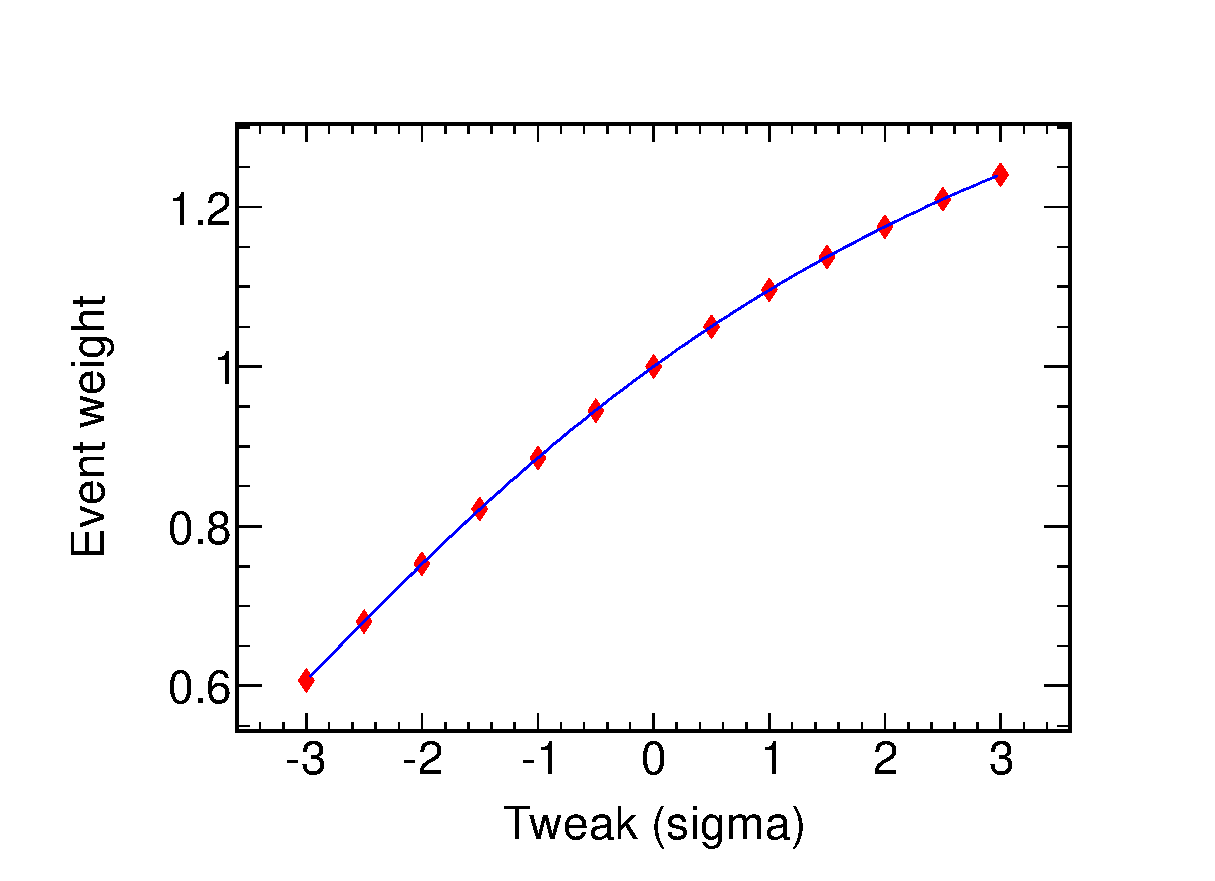
\includegraphics[width=25pc]{./images/spectrum_tweaked/ExampleSpline}
%
\includegraphics[width=15pc]{./images/placeholder}
%\caption {
%Example of a cross-section spline; this shows the event weights obtained by tweaking $M_{A}^{QE}$
%for $\nu_{\mu}$-CCQE events in the bin with reconstructed energy 0.75-0.8 GeV and 
%true energy 0.6-0.7 GeV.
%}
%\label{fig:example_spline}
%\end{figure}
%
%....................................................................................................................


\subsection {Evaluation of effects of systematic parameters on the predicted single $\mu$-like ring reconstructed energy spectrum}
\label{sec:systematics:evaluation}

In this section, we present the effects of the systematics described in Sec.\ \ref{sec:systematics:inputs}
on the predicted number of single $\mu$-like ring events and the predicted reconstructed energy spectrum in SuperK.
These effects are shown both without oscillations and with oscillations with
$\sin^{2}\theta_{23}$ = 0.5 and $|\Delta m^{2}_{32}|$ = 2.4$\times$10$^{-3}$ eV$^{2}$/c$^{4}$, the values shown in Tab.\
\ref{tab:pdg2012non23} for $\sin^{2}\theta_{13}$, $\sin^{2}\theta_{12}$ and $\Delta m^{2}_{21}$,
and $\delta_{CP}$=0. The normal mass hierarchy is assumed.
All results are generated for an integrated exposure of 6.5700$\times$10$^{20}$ POT and
the BANFF-tuned MC templates are used.

The effects of systematic uncertainties on the predicted number of events are summarised in Tab.\ \ref{tab:nsk_systematic_table_summary}, 
both for no oscillations and for oscillations with the typical parameter values given above.
In this table, systematic parameters are grouped into five categories and all parameter correlations are taken into account.
Percentage uncertainties are given for both the BANFF prefit and postfit errors.
The individual effect of each parameter is also presented in Tab.\ \ref{tab:nsk_systematic_table}, in which the correlations
between parameters are necessarily ignored.

The effects of the combined systematic uncertainties on the reconstructed energy spectrum of single $\mu$-like ring events
is shown in Fig.\ \ref{fig:1Rmu_error_envelope_total} for the typical oscillation scenario used.
This plot shows the total error envelope for the 1 $\mu$-like ring event reconstructed energy spectrum; this is calculated
as the $\pm$1$\sigma$ spread of bin contents from 100k toy MC experiments generated with randomized systematic parameters.
In Fig.\ \ref{fig:1Rmu_error_envelope_total}, all systematic parameters were considered and their correlations were taken
into account.

Figs.\ \ref{fig:1Rmu_error_ratio_to_nominal_unosc} and \ref{fig:1Rmu_error_ratio_to_nominal_osc}
show the effect of the systematic error, relative to the statistical error
at the Run 1-4 exposure, for the no oscillation and oscillation cases respectively.
It can be seen that the statistical error dominates at all energies.

Figs.\ \ref{fig:1Rmu_systematics_spread_by_group_unosc} and \ref{fig:1Rmu_systematics_spread_by_group_osc}
show the effect of the four categories of systematic error,
relative to the total systematic error, for the no oscillation and oscillation cases respectively.
It can be seen that the SuperK detector + FSI + SI and
uncorrelated cross section systematics dominate the oscillation dip region.

Detailed studies showing the effects of individual systematics on the expected number of
single $\mu$-like ring events are shown in \cite{OurRun1234DisappAnalysisSupplement}.

The individual effect of each systematic parameter on the best-fit values of $\sin^{2}\theta_{23}$ and $|\Delta m^{2}_{32}|$ 
for the normal hierarchy was quantified by making a toy MC experiment with no statistical fluctuations and a +1$\sigma$ tweak of a 
single systematic parameter. A fit for only $\sin^2\theta_{23}$ and $|\Delta m^2_{32}|$, with systematics fixed
are their nominal values,
was made of that experiment, and the +1$\sigma$ effect of that systematic parameter on the 
best-fit values of $\sin^{2}\theta_{23}$ and $|\Delta m^{2}_{32}|$ was taken to be the difference between the best-fit values from 
the experiment with the +1$\sigma$ tweak and an experiment with nominal values of the systematics. Similarly, the -1$\sigma$ effect of that 
parameter was the difference between the best-fit values from an experiment with a -1$\sigma$ tweak and an experiment with 
nominal values of the systematics. This procedure was repeated for each systematic parameter in turn.
For systematic parameters which are correlated, this procedure was repeated twice, both respecting and ignoring correlations.
The study is repeated at multiple input points in the $\sin^{2}\theta_{23}$-$|\Delta m^{2}_{32}|$ plane.

An estimate of the order of the effect of systematics is given in Tabs.\ \ref{tab:star_summary_by_mixing} and
\ref{tab:star_summary_by_mass}, ordered by the effect on $\sin^2\theta_{23}$ and $|\Delta m^2_{32}|$ respectively.
To make this estimate, the systematic effect is compared with the statistical error for the
specific values of $\sin^2\theta_{23}$ and $|\Delta m^2_{32}|$.
The statistical error was evaluated using 10k toy MC datasets with no systematic fluctuations at each input point, 
with each dataset being fitted for only $\sin^\theta_{23}$ and $|\Delta m^2_{32}|$.
For each systematic, the largest effect seen in the study is given, 
whether that is from +1$\sigma$ or -1$\sigma$, including or neglecting correlations,
and from any true values of $\sin^{2}\theta_{23}$ and $|\Delta m^{2}_{32}|$ in the study.


% ..................

\begin{table}[htb]
\centering
\begin{tabular}{| c | D{.}{.}{-1} | D{.}{.}{-1} |}
\hline
%  {\bf Source of uncertainty}    & \multicolumn{1}{c|}{{\bf ${\delta}N_{SK}$/$N_{SK}$}} & \multicolumn{1}{c|}{{\bf ${\delta}N_{SK}$/$N_{SK}$}}\\
  {\bf Source of uncertainty}    & \multicolumn{1}{c|}{{\bf ${\delta}N_{SK}$/$ <N_{SK} >$}} & \multicolumn{1}{c|}{{\bf ${\delta}N_{SK}$/$<N_{SK}>$}}\\
                                 & \multicolumn{1}{c|}{($\beta=0$)} & \multicolumn{1}{c|}{($\beta=1$)}\\
\hline
  SuperK detector    				& 5.05\%                         & 3.03\%                        \\
  FSI + SI + PN 					& 4.34\%				& 2.45\%			\\
  SuperK detector + FSI + SI + PN     & 6.66\%                         & 3.90\%                        \\
\hline
  BANFF (prefit)                 &  12.37\%                        & 12.91\%                       \\
  BANFF (postfit)                & 9.72\%                         & 10.29\%                        \\
\hline
  BANFF (Non-oxygen, postfit)    	& 3.40\%         	         & 3.02\%                        \\
  BANFF (Oxygen-specific postfit) 	& 9.24\%                    & 10.14\%                        \\
  MEC (Oxygen-specific postfit)	   	& 8.86\%                        	 & 9.28\%                        \\
\hline
  Oscillation parameters         & 4.72\%                         & 13.38\%                       \\
\hline
  Total (BANFF prefit)           &  14.96\%                        & 18.60\%                       \\
  Total (BANFF postfit)          & 12.75\%                         & 17.21\%                       \\
\hline
\end{tabular}
\caption{
 Effect of 1$\sigma$ variations of the groups of systematics parameters on total number of
 1-ring electron-like events in the reverse-horn current sample.
 The BANFF parameters considered to be oxygen-specific are Oxygen MEC normalisation, Fermi Energy, Binding Energy, CC Coherent Normalisation,
 NC Coherent normalization and the nue/numu normalisation. 
The effect of each group of systematics is computed as the standard deviation divided by the mean of the distribution
of the total number of superK events.
\NumToys are performed.
% \newline
%{\bf TO UPDATE}
%\newline
}
\label{tab:nsk_systematic_table_summary}
\end{table}


%..................

\begin{table}
\centering
\begin{tabular}{| c || D{.}{.}{-1} | D{.}{.}{-1} || D{.}{.}{-1} | D{.}{.}{-1} |}
\hline
  Source of uncertainty        &  \multicolumn {2}{c||}{${\delta}N_{SK}$/$N_{SK}$} & \multicolumn {2}{c|}{${\delta}N_{SK}$/$N_{SK}$} \\
                               &  \multicolumn {2}{c||}{(no oscillation)}          & \multicolumn {2}{c|}{(oscillations with typical params)} \\
                               & \multicolumn {1}{c|}{BANFF prefit} & \multicolumn {1}{c||}{BANFF postfit} & \multicolumn {1}{c|}{BANFF prefit} & \multicolumn {1}{c|}{BANFF postfit} \\
\hline
               $f_{E; r}^{SK}$ &               0 &               0 &               0 &               0  \\   
           $f_{0; r}^{SK+FSI}$ &            0.09 &           0.098 &            0.15 &            0.18  \\   
           $f_{1; r}^{SK+FSI}$ &             1.8 &             1.9 &            0.68 &            0.74  \\   
           $f_{2; r}^{SK+FSI}$ &             0.4 &            0.43 &            0.92 &             1.0  \\   
           $f_{3; r}^{SK+FSI}$ &             2.4 &             2.1 &             4.6 &             4.0  \\   
           $f_{4; r}^{SK+FSI}$ &           0.017 &           0.016 &            0.25 &            0.27  \\   
           $f_{5; r}^{SK+FSI}$ &             1.1 &             0.9 &             3.8 &             3.2  \\   
\hline
         $f_{0; t, r}^{banff}$ &            0.36 &            0.27 &            0.85 &            0.66  \\   
         $f_{1; t, r}^{banff}$ &             1.0 &            0.74 &            0.67 &             0.5  \\   
         $f_{2; t, r}^{banff}$ &             1.9 &             1.3 &            0.12 &           0.085  \\   
         $f_{3; t, r}^{banff}$ &             2.3 &             1.6 &             0.3 &            0.22  \\   
         $f_{4; t, r}^{banff}$ &             3.4 &             2.4 &             2.2 &             1.6  \\   
         $f_{5; t, r}^{banff}$ &             1.0 &            0.66 &             1.8 &             1.2  \\   
         $f_{6; t, r}^{banff}$ &            0.63 &            0.39 &             1.7 &             1.1  \\   
         $f_{7; t, r}^{banff}$ &            0.33 &             0.2 &             1.0 &            0.65  \\   
         $f_{8; t, r}^{banff}$ &            0.41 &            0.22 &             1.3 &            0.74  \\   
         $f_{9; t, r}^{banff}$ &            0.19 &           0.077 &            0.65 &            0.27  \\   
        $f_{10; t, r}^{banff}$ &           0.051 &           0.019 &            0.17 &           0.066  \\   
        $f_{11; t, r}^{banff}$ &           0.061 &            0.05 &           0.035 &            0.03  \\   
        $f_{12; t, r}^{banff}$ &           0.061 &           0.049 &           0.049 &            0.04  \\   
        $f_{13; t, r}^{banff}$ &           0.085 &           0.067 &            0.16 &            0.13  \\   
        $f_{14; t, r}^{banff}$ &             0.1 &            0.08 &            0.27 &            0.22  \\   
        $f_{15; t, r}^{banff}$ &           0.078 &            0.06 &            0.25 &             0.2  \\   
        $f_{16; t, r}^{banff}$ &            25.0 &             3.4 &            18.0 &             2.8  \\   
        $f_{17; t, r}^{banff}$ &             2.8 &             1.1 &             6.7 &             2.4  \\   
        $f_{18; t, r}^{banff}$ &             7.9 &             5.9 &             4.2 &             3.3  \\   
        $f_{19; t, r}^{banff}$ &             1.4 &            0.55 &             3.9 &             1.6  \\   
        $f_{20; t, r}^{banff}$ &            0.36 &            0.16 &             1.2 &            0.53  \\   
        $f_{21; t, r}^{banff}$ &             3.7 &             1.5 &             4.9 &             2.0  \\   
        $f_{22; t, r}^{banff}$ &             1.7 &            0.47 &             5.4 &             1.6  \\   
\hline
                $f_{pF; t, r}$ &           0.063 &           0.065 &            0.13 &            0.13  \\   
                $f_{SF; t, r}$ &            0.82 &            0.82 &            0.24 &            0.26  \\   
            $f_{Wshape; t, r}$ &            0.12 &           0.072 &             0.4 &            0.26  \\   
        $f_{CCothShape; t, r}$ &            0.28 &             0.3 &            0.78 &            0.89  \\   
    $f_{\pi-less\Delta; t, r}$ &             3.2 &             2.6 &             5.6 &             4.5  \\   
             $f_{bindE; t, r}$ &             0.5 &            0.43 &            0.24 &             0.2  \\   
                $f_{CCcoh; t}$ &            0.54 &            0.58 &            0.81 &            0.93  \\   
           $f_{NC1\pi^\pm; t}$ &            0.31 &            0.21 &             1.1 &            0.75  \\   
                $f_{NCoth; t}$ &            0.25 &            0.24 &            0.85 &            0.85  \\   
              $f_{CC\nu_e; t}$ &         0.00051 &          0.0005 &          0.0077 &          0.0081  \\   
          $f_{CC\bar{\nu}; t}$ &            0.61 &            0.61 &             1.2 &             1.2  \\   
\hline
         $\sin^2(\theta_{13})$ &               0 &               0 &           0.070 &           0.078  \\   
         $\sin^2(\theta_{12})$ &               0 &               0 &           0.040 &           0.036  \\   
             $\Delta m^2_{21}$ &               0 &               0 &           0.027 &           0.025  \\   
                 $\delta_{CP}$ &               0 &               0 &            0.21 &            0.19  \\   

 


\hline
\end{tabular}
\caption{
  Effects of 1$\sigma$ systematic parameter variations on
  the number of 1 $\mu$-like ring events,
  computed
  for no oscillations and
  for oscillations with
  $\sin^{2}\theta_{23}$=0.5, $|\Delta m^{2}_{32}|$=2.4$\times$10$^{-3}$ eV$^{2}$/c$^{4}$, the values shown in Tab.\
  \ref{tab:pdg2012non23} for $\sin^{2}\theta_{13}$, $\sin^{2}\theta_{12}$ and $\Delta m^{2}_{21}$,
  and $\delta_{CP}$=0. Correlations are ignored for this table. The normal mass hierarchy is assumed.
  The numbers shown were calculated for an exposure of 6.5700$\times$10$^{20}$ POT and BANFF-tuned MC templates were used.
}
\label{tab:nsk_systematic_table}
\end{table}


%..................

\begin{figure*}[htb]
\center
\includegraphics[width=30pc]{{./images/spectrum_tweaked/all_envelope_per_50MeV_sinsqtheta12_0.312,13_0.025,23_0.500,dcp_0.000,dmsq_Normal12_0.00007500,23_0.002400eV2}.eps}
\caption {
  Total error envelope of the 1 $\mu$-like ring event reconstructed energy spectrum,
  for oscillations with
  $\sin^{2}\theta_{23}$=0.5 and $|\Delta m^{2}_{32}|$=2.4$\times$10$^{-3}$ eV$^{2}$/c$^{4}$, the values shown in 
  Tab.\ \ref{tab:pdg2012non23} for $\sin^{2}\theta_{13}$, $\sin^{2}\theta_{12}$ and $\Delta m^{2}_{21}$,
  and $\delta_{CP}$=0. The normal mass hierarchy is assumed.
  The numbers shown were calculated for an exposure of 6.5700$\times$10$^{20}$ POT.
  BANFF-tuned MC templates were used.
  The error envelope was calculated as the $\pm$1$\sigma$ spread of bin contents using an ensemble of 100k toy MC experiments
  generated with randomized systematic parameters.
  All systematic parameters were considered and their correlations were taken into account.
}
\label{fig:1Rmu_error_envelope_total}
\end{figure*}

%..................

\begin{figure*}[htb]
\begin{minipage}[t]{0.48\linewidth}
\center
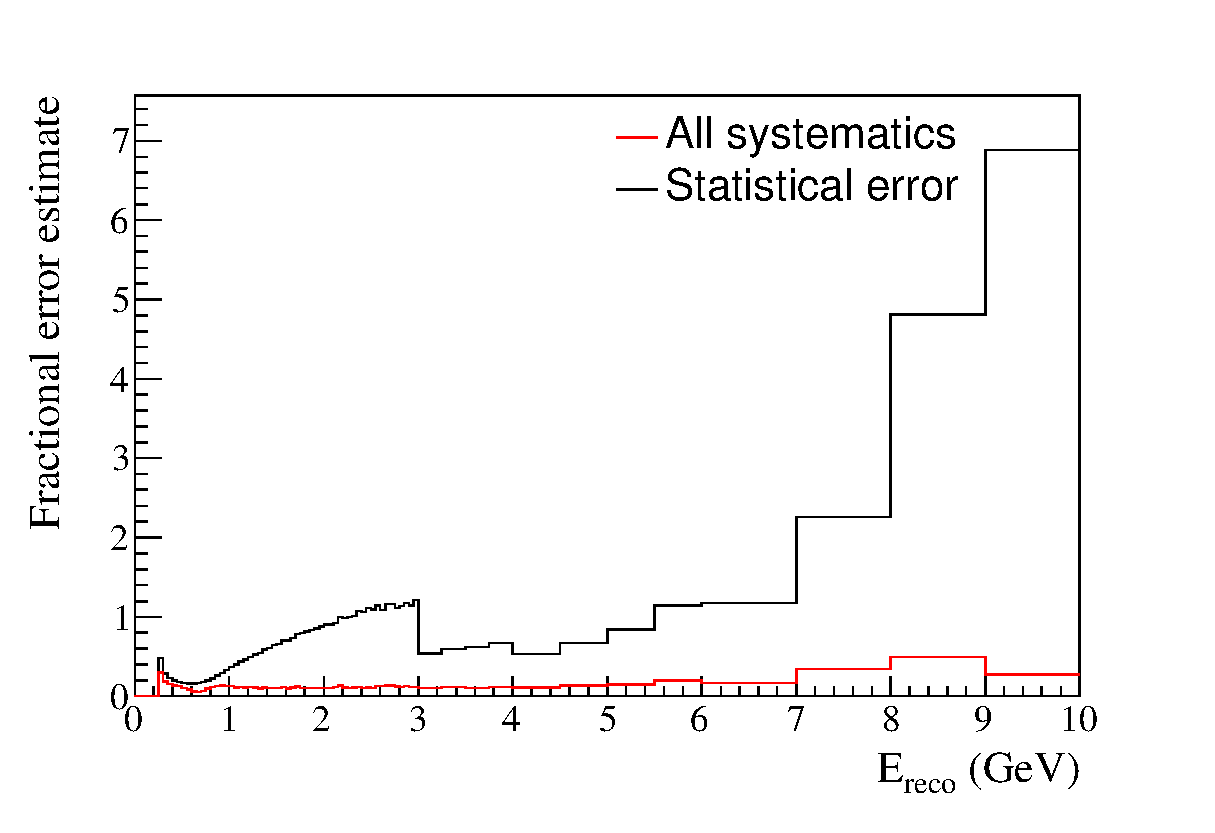
\includegraphics[width=20pc]{./images/spectrum_tweaked/unoscillated_statistical_systematic_sizes.eps}
\caption {
  Comparative size of systematic and statistical error effects per bin.
  100k toy MC experiments were generated with randomized systematic parameters and the 1$\sigma$ spread of bin contents was calculated.
  The fractional systematic error is estimated as the 1$\sigma$ spread divided by the expected number of events in each bin.
  The fractional statistical error is estimated as the inverse square root of the number of events in each bin at 6.5700$\times$10$^{20}$ POT.
  BANFF tuned MC templates were used.
  All systematic parameters were considered and their correlations were taken into account.
  No oscillations were applied.
}
\label{fig:1Rmu_error_ratio_to_nominal_unosc}
\end{minipage}
\hspace{0.06\linewidth}
\begin{minipage}[t]{0.48\linewidth}
\center
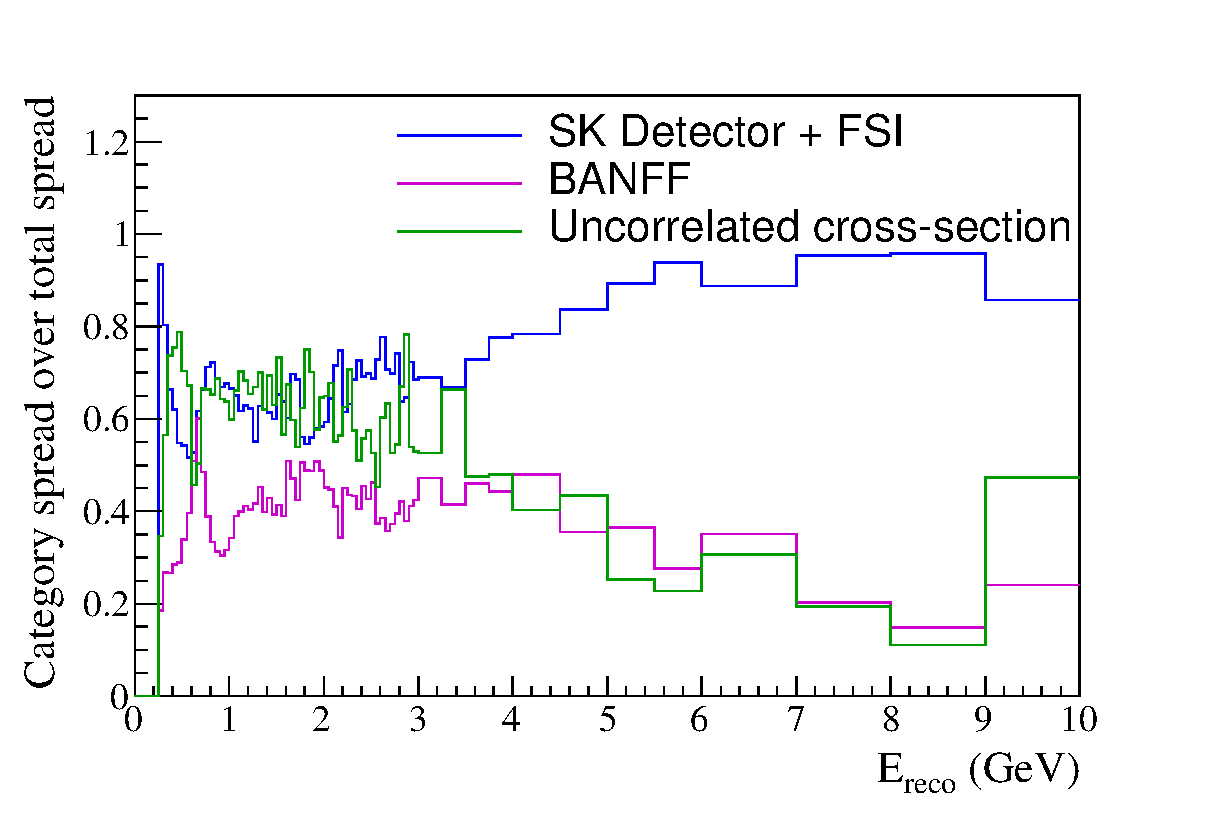
\includegraphics[width=20pc]{./images/spectrum_tweaked/unoscillated_systematic_spread_ratios.eps}
\caption {
  Ratio of event-per-bin 1$\sigma$ spread with individual systematic categories randomized, to the equivalent spread with all systematics randomized.
  100k toy MC experiments each were generated with different groups of systematics randomized, and with all systematics randomized, and the 1$\sigma$ spread of bin contents was calculated.
  BANFF tuned MC templates were used.
  No oscillations were applied.
}
\label{fig:1Rmu_systematics_spread_by_group_unosc}
\end{minipage}
\end{figure*}

\begin{figure*}[htb]
\begin{minipage}[t]{0.48\linewidth}
\center
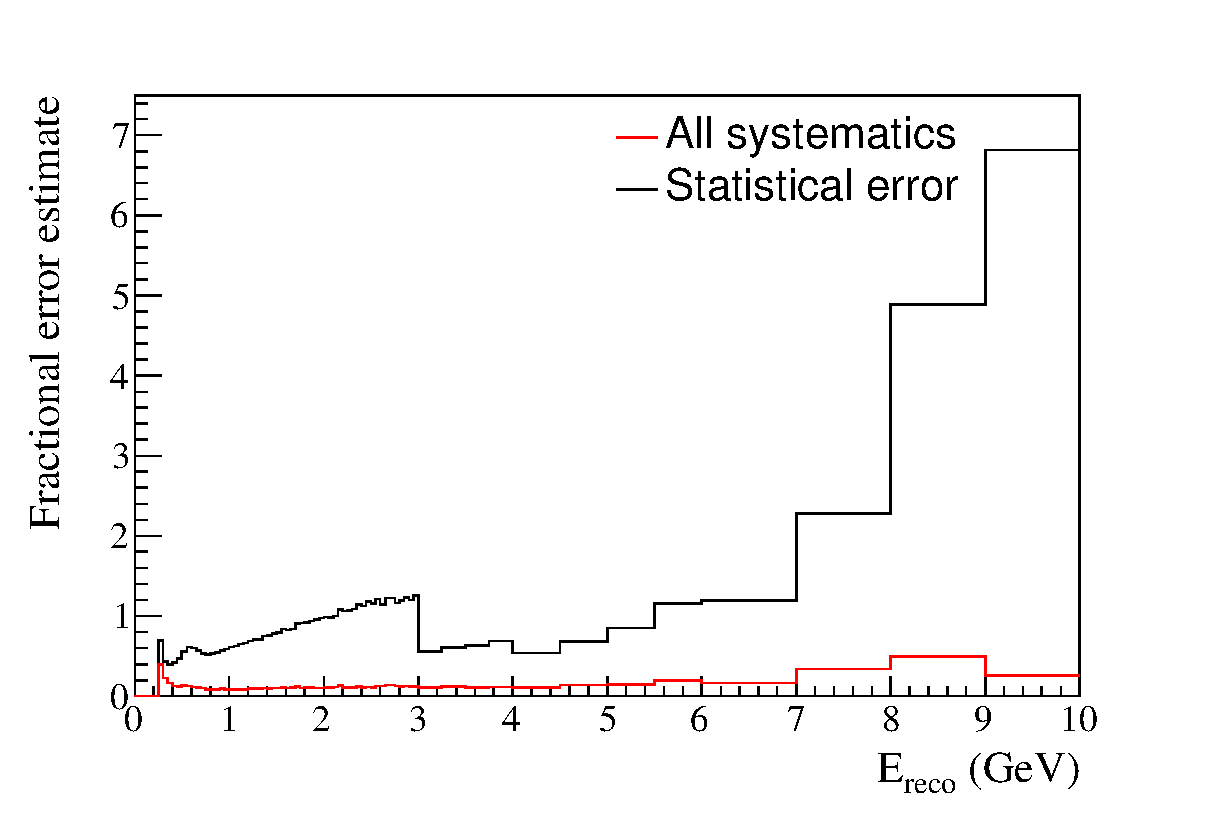
\includegraphics[width=20pc]{./images/spectrum_tweaked/oscillated_statistical_systematic_sizes.eps}
\caption {
  As in Fig. \ref{fig:1Rmu_error_ratio_to_nominal_unosc}, but with oscillations applied for $\sin^{2}\theta_{23}$=0.5, $|\Delta m^{2}_{32}|$=2.4$\times$10$^{-3}$ eV$^{2}$/c$^{4}$, the values shown in
  Tab.\ \ref{tab:pdg2012non23} for $\sin^{2}\theta_{13}$, $\sin^{2}\theta_{12}$ and $\Delta m^{2}_{21}$,
  and $\delta_{CP}$=0. The normal mass hierarchy is assumed. 
}
\label{fig:1Rmu_error_ratio_to_nominal_osc}
\end{minipage}
\hspace{0.06\linewidth}
\begin{minipage}[t]{0.48\linewidth}
\center
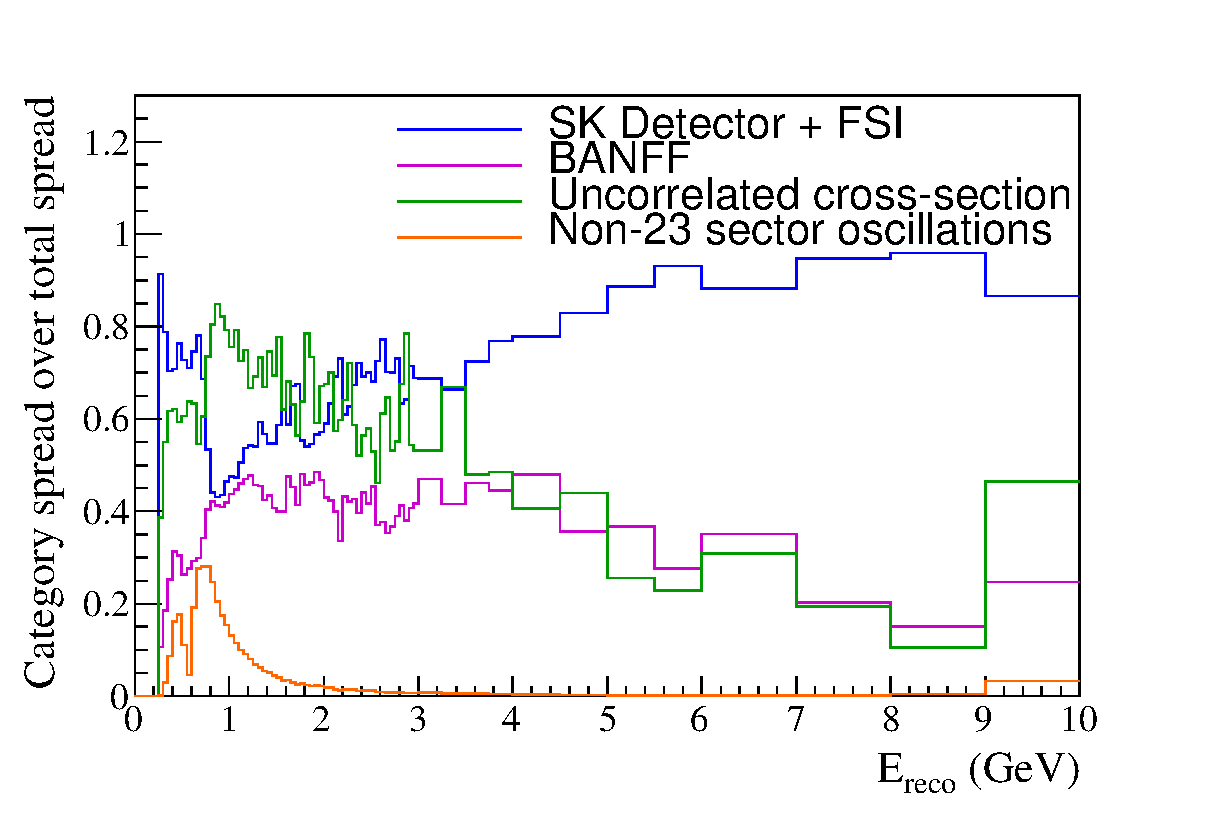
\includegraphics[width=20pc]{./images/spectrum_tweaked/oscillated_systematic_spread_ratios.eps}
\caption {
  As in Fig. \ref{fig:1Rmu_systematics_spread_by_group_unosc}, but with oscillations applied for $\sin^{2}\theta_{23}$=0.5, $|\Delta m^{2}_{32}|$=2.4$\times$10$^{-3}$ eV$^{2}$/c$^{4}$, the values shown in
  Tab.\ \ref{tab:pdg2012non23} for $\sin^{2}\theta_{13}$, $\sin^{2}\theta_{12}$ and $\Delta m^{2}_{21}$,
  and $\delta_{CP}$=0. The normal mass hierarchy is assumed. 
}
\label{fig:1Rmu_systematics_spread_by_group_osc}
\end{minipage}
\end{figure*}

%..................

\begin{table}
\small
\centering
\begin{tabular}{| c | c | c |}
\hline
 Parameter               &  $\frac{\delta_{syst} sin^2\overline{\theta_{23}}}{\delta_{stat} sin^2\overline{\theta_{23}}}$   &  $\frac{\delta_{syst}|\overline{\Delta m^2_{32}}| (eV^{2}/c^{4})}{\delta_{stat} |\overline{\Delta m^2_{32}}| (eV^{2}/c^{4})}$ \\
\hline
                               SKDet + FSI/SI  5; $E_r$ =  0.00 - 30.00 GeV; all NC; RHC & 1.040 & 0.225 \\ \hline 
                                       Meson exchange current normalisation for $^{16}$O & 0.918 & 0.127 \\ \hline 
                                                  CC coherent for $^{16}$O normalisation & 0.491 & 0.028 \\ \hline 
                            C$^{A}_{5}$ nucleon to $\Delta$ transition axial form factor & 0.422 & 0.024 \\ \hline 
                                                                    SK energy scale; RHC & 0.383 & 0.101 \\ \hline 
                                                                  NC other normalisation & 0.347 & 0.029 \\ \hline 
                               RHC $\bar{\nu_\mu}$ flux normalisation, E = 0.7 - 1.0 GeV & 0.326 & 0.048 \\ \hline 
       SKDet + FSI/SI  3; $E_r$ =  0.00 - 30.00 GeV; $\overset{(-)}{\nu_\mu}$ CCnQE; RHC & 0.315 & 0.022 \\ \hline 
                                             Scale of isospin 1/2 nonresonant background & 0.315 & 0.012 \\ \hline 
                                          Resonance-production axial-mass scaling factor & 0.247 & 0.011 \\ \hline 
                                                             Fermi momentum for $^{16}$O & 0.230 & 0.024 \\ \hline 
                               RHC $\bar{\nu_\mu}$ flux normalisation, E = 0.0 - 0.4 GeV & 0.228 & 0.021 \\ \hline 
         SKDet + FSI/SI  1; $E_r$ =  0.40 - 1.10 GeV; $\overset{(-)}{\nu_\mu}$ CCQE; RHC & 0.225 & 0.023 \\ \hline 
            SKDet + FSI/SI  4; $E_r$ =  0.00 - 30.00 GeV; $\overset{(-)}{\nu_e}$ CC; RHC & 0.211 & 0.009 \\ \hline 
                               RHC $\bar{\nu_\mu}$ flux normalisation, E = 1.0 - 1.5 GeV & 0.202 & 0.016 \\ \hline 
                                                          CCQE axial-mass scaling factor & 0.200 & 0.021 \\ \hline 
                               RHC $\bar{\nu_\mu}$ flux normalisation, E = 0.4 - 0.5 GeV & 0.190 & 0.030 \\ \hline 
                                     RHC $\nu_\mu$ flux normalisation, E = 1.0 - 1.5 GeV & 0.150 & 0.009 \\ \hline 
                               RHC $\bar{\nu_\mu}$ flux normalisation, E = 0.6 - 0.7 GeV & 0.142 & 0.009 \\ \hline 
         SKDet + FSI/SI  0; $E_r$ =  0.00 - 0.40 GeV; $\overset{(-)}{\nu_\mu}$ CCQE; RHC & 0.116 & 0.006 \\ \hline 
                               RHC $\bar{\nu_\mu}$ flux normalisation, E = 0.5 - 0.6 GeV & 0.115 & 0.025 \\ \hline 
                                     RHC $\nu_\mu$ flux normalisation, E = 0.7 - 1.0 GeV & 0.113 & 0.006 \\ \hline 
                               RHC $\bar{\nu_\mu}$ flux normalisation, E = 1.5 - 2.5 GeV & 0.108 & 0.005 \\ \hline 
                                     RHC $\nu_\mu$ flux normalisation, E = 0.0 - 0.7 GeV & 0.100 & 0.009 \\ \hline 
                                                                          CC other shape & 0.096 & 0.003 \\ \hline 
                                     RHC $\nu_\mu$ flux normalisation, E = 1.5 - 2.5 GeV & 0.087 & 0.006 \\ \hline 
                                    RHC $\nu_\mu$ flux normalisation, E = 2.5 - 30.0 GeV & 0.085 & 0.004 \\ \hline 
        SKDet + FSI/SI  2; $E_r$ =  1.10 - 30.00 GeV; $\overset{(-)}{\nu_\mu}$ CCQE; RHC & 0.070 & 0.005 \\ \hline 
                                                             Binding energy for $^{16}$O & 0.063 & 0.007 \\ \hline 
                               RHC $\bar{\nu_\mu}$ flux normalisation, E = 2.5 - 3.5 GeV & 0.051 & 0.001 \\ \hline 
                               RHC $\bar{\nu_\mu}$ flux normalisation, E = 3.5 - 5.0 GeV & 0.021 & 0.002 \\ \hline 
                                                               NC coherent normalisation & 0.019 & 0.000 \\ \hline 
                              RHC $\bar{\nu_\mu}$ flux normalisation, E = 7.0 - 30.0 GeV & 0.009 & 0.000 \\ \hline 
                                                              CC $\nu_{e}$ normalisation & 0.008 & 0.000 \\ \hline 
                               RHC $\bar{\nu_\mu}$ flux normalisation, E = 5.0 - 7.0 GeV & 0.007 & 0.000 \\ \hline 
                                      RHC $\nu_e$ flux normalisation, E = 2.5 - 30.0 GeV & 0.006 & 0.000 \\ \hline 
                                       RHC $\nu_e$ flux normalisation, E = 0.0 - 2.5 GeV & 0.004 & 0.000 \\ \hline 
                                RHC $\bar{\nu_e}$ flux normalisation, E = 4.0 - 30.0 GeV & 0.003 & 0.000 \\ \hline 
                                 RHC $\bar{\nu_e}$ flux normalisation, E = 2.5 - 4.0 GeV & 0.002 & 0.000 \\ \hline 
                                 RHC $\bar{\nu_e}$ flux normalisation, E = 1.5 - 2.5 GeV & 0.001 & 0.000 \\ \hline 
                                 RHC $\bar{\nu_e}$ flux normalisation, E = 0.8 - 1.5 GeV & 0.000 & 0.000 \\ \hline 
                                 RHC $\bar{\nu_e}$ flux normalisation, E = 0.5 - 0.7 GeV & 0.000 & 0.000 \\ \hline 
                                 RHC $\bar{\nu_e}$ flux normalisation, E = 0.0 - 0.5 GeV & 0.000 & 0.000 \\ \hline 
                                 RHC $\bar{\nu_e}$ flux normalisation, E = 0.7 - 0.8 GeV & 0.000 & 0.000 \\ \hline 
                            
\hline
\end{tabular}
\caption{
  Maximum deviations, as a fraction of statistical error at the oscillation
  parameter grid point, from the input values of fits for only $\sin^2\overline{\theta_{23}}$ and $|\overline{\Delta m^2_{32}}|$ to datasets with 
  $\pm$1 sigma individual systematic variations at a range of 23-sector oscillation points.
  $|\overline{\Delta m^2_{32}}|$ values of
  2.0$\times$10$^{-3}$ eV$^{2}$/c$^{4}$,
  2.5$\times$10$^{-3}$ eV$^{2}$/c$^{4}$, and
  3.0$\times$10$^{-3}$ eV$^{2}$/c$^{4}$
  are used with each of
  $\sin^2\overline{\theta_{23}} = $ 
  0.370, 0.500, 0.524, 0.650.
  All other oscillation parameters are fixed at the values in table~\ref{tab:osc_params_fixed_values_reactor}.
  These maximum deviations usually occur at maximum disappearance, where the statistical error is smaller, as explained in
  Sec.~\ref{sec:validation}. The values are sorted by the size of the deviation in $\sin^2\overline{\theta_{23}}$.
}
\label{tab:star_summary_by_mixing}
\end{table}

\begin{table}
\small
\centering
\begin{tabular}{| c | c | c |}
\hline
 Parameter               &  $\frac{\delta_{syst} sin^2\overline{\theta_{23}}}{\delta_{stat} sin^2\overline{\theta_{23}}}$   &  $\frac{\delta_{syst}|\overline{\Delta m^2_{32}}| (eV^{2}/c^{4})}{\delta_{stat} |\overline{\Delta m^2_{32}}| (eV^{2}/c^{4})}$ \\
\hline
                                      SKDet + FSI/SI  5; $E_r$ =  0.00 - 30.00 GeV; all NC; RHC & 1.040 & 0.225 \\ \hline 
                                              Meson exchange current normalisation for $^{16}$O & 0.918 & 0.127 \\ \hline 
                                                                           SK energy scale; RHC & 0.383 & 0.101 \\ \hline 
                                      RHC $\bar{\nu_\mu}$ flux normalisation, E = 0.7 - 1.0 GeV & 0.326 & 0.048 \\ \hline 
                                      RHC $\bar{\nu_\mu}$ flux normalisation, E = 0.4 - 0.5 GeV & 0.190 & 0.030 \\ \hline 
                                                                         NC other normalisation & 0.347 & 0.029 \\ \hline 
                                                         CC coherent for $^{16}$O normalisation & 0.491 & 0.028 \\ \hline 
                                      RHC $\bar{\nu_\mu}$ flux normalisation, E = 0.5 - 0.6 GeV & 0.115 & 0.025 \\ \hline 
                                   C$^{A}_{5}$ nucleon to $\Delta$ transition axial form factor & 0.422 & 0.024 \\ \hline 
                                                                    Fermi momentum for $^{16}$O & 0.230 & 0.024 \\ \hline 
                SKDet + FSI/SI  1; $E_r$ =  0.40 - 1.10 GeV; $\overset{(-)}{\nu_\mu}$ CCQE; RHC & 0.225 & 0.023 \\ \hline 
              SKDet + FSI/SI  3; $E_r$ =  0.00 - 30.00 GeV; $\overset{(-)}{\nu_\mu}$ CCnQE; RHC & 0.315 & 0.022 \\ \hline 
                                                                 CCQE axial-mass scaling factor & 0.200 & 0.021 \\ \hline 
                                      RHC $\bar{\nu_\mu}$ flux normalisation, E = 0.0 - 0.4 GeV & 0.228 & 0.021 \\ \hline 
                                      RHC $\bar{\nu_\mu}$ flux normalisation, E = 1.0 - 1.5 GeV & 0.202 & 0.016 \\ \hline 
                                                    Scale of isospin 1/2 nonresonant background & 0.315 & 0.012 \\ \hline 
                                                 Resonance-production axial-mass scaling factor & 0.247 & 0.011 \\ \hline 
                                      RHC $\bar{\nu_\mu}$ flux normalisation, E = 0.6 - 0.7 GeV & 0.142 & 0.009 \\ \hline 
                   SKDet + FSI/SI  4; $E_r$ =  0.00 - 30.00 GeV; $\overset{(-)}{\nu_e}$ CC; RHC & 0.211 & 0.009 \\ \hline 
                                            RHC $\nu_\mu$ flux normalisation, E = 0.0 - 0.7 GeV & 0.100 & 0.009 \\ \hline 
                                            RHC $\nu_\mu$ flux normalisation, E = 1.0 - 1.5 GeV & 0.150 & 0.009 \\ \hline 
                                                                    Binding energy for $^{16}$O & 0.063 & 0.007 \\ \hline 
                                            RHC $\nu_\mu$ flux normalisation, E = 1.5 - 2.5 GeV & 0.087 & 0.006 \\ \hline 
                SKDet + FSI/SI  0; $E_r$ =  0.00 - 0.40 GeV; $\overset{(-)}{\nu_\mu}$ CCQE; RHC & 0.116 & 0.006 \\ \hline 
                                            RHC $\nu_\mu$ flux normalisation, E = 0.7 - 1.0 GeV & 0.113 & 0.006 \\ \hline 
                                      RHC $\bar{\nu_\mu}$ flux normalisation, E = 1.5 - 2.5 GeV & 0.108 & 0.005 \\ \hline 
               SKDet + FSI/SI  2; $E_r$ =  1.10 - 30.00 GeV; $\overset{(-)}{\nu_\mu}$ CCQE; RHC & 0.070 & 0.005 \\ \hline 
                                           RHC $\nu_\mu$ flux normalisation, E = 2.5 - 30.0 GeV & 0.085 & 0.004 \\ \hline 
                                                                                 CC other shape & 0.096 & 0.003 \\ \hline 
                                      RHC $\bar{\nu_\mu}$ flux normalisation, E = 3.5 - 5.0 GeV & 0.021 & 0.002 \\ \hline 
                                      RHC $\bar{\nu_\mu}$ flux normalisation, E = 2.5 - 3.5 GeV & 0.051 & 0.001 \\ \hline 
                                      RHC $\bar{\nu_\mu}$ flux normalisation, E = 5.0 - 7.0 GeV & 0.007 & 0.000 \\ \hline 
                                                                      NC coherent normalisation & 0.019 & 0.000 \\ \hline 
                                     RHC $\bar{\nu_\mu}$ flux normalisation, E = 7.0 - 30.0 GeV & 0.009 & 0.000 \\ \hline 
                                                                     CC $\nu_{e}$ normalisation & 0.008 & 0.000 \\ \hline 
                                             RHC $\nu_e$ flux normalisation, E = 2.5 - 30.0 GeV & 0.006 & 0.000 \\ \hline 
                                              RHC $\nu_e$ flux normalisation, E = 0.0 - 2.5 GeV & 0.004 & 0.000 \\ \hline 
                                        RHC $\bar{\nu_e}$ flux normalisation, E = 2.5 - 4.0 GeV & 0.002 & 0.000 \\ \hline 
                                       RHC $\bar{\nu_e}$ flux normalisation, E = 4.0 - 30.0 GeV & 0.003 & 0.000 \\ \hline 
                                        RHC $\bar{\nu_e}$ flux normalisation, E = 1.5 - 2.5 GeV & 0.001 & 0.000 \\ \hline 
                                        RHC $\bar{\nu_e}$ flux normalisation, E = 0.0 - 0.5 GeV & 0.000 & 0.000 \\ \hline 
                                        RHC $\bar{\nu_e}$ flux normalisation, E = 0.5 - 0.7 GeV & 0.000 & 0.000 \\ \hline 
                                        RHC $\bar{\nu_e}$ flux normalisation, E = 0.7 - 0.8 GeV & 0.000 & 0.000 \\ \hline 
                                        RHC $\bar{\nu_e}$ flux normalisation, E = 0.8 - 1.5 GeV & 0.000 & 0.000 \\ \hline 
\hline
\end{tabular}
\caption{
  Maximum deviations, as a fraction of statistical error at the oscillation
  parameter grid point, from the input values of fits for only $\sin^2\overline{\theta_{23}}$ and $|\overline{\Delta m^2_{32}}|$ to datasets with 
  $\pm$1 sigma individual systematic variations at a range of 23-sector oscillation points.
  $|\overline{\Delta m^2_{32}}|$ values of
  2.0$\times$10$^{-3}$ eV$^{2}$/c$^{4}$,
  2.5$\times$10$^{-3}$ eV$^{2}$/c$^{4}$, and
  3.0$\times$10$^{-3}$ eV$^{2}$/c$^{4}$
  are used with each of
  $\sin^2\overline{\theta_{23}} = $ 
  0.370, 0.500, 0.524, 0.650.
  All other oscillation parameters are fixed at the values in table~\ref{tab:osc_params_fixed_values_reactor}.
  These maximum deviations usually occur at maximum disappearance, where the statistical error is smaller, as explained in
  Sec.~\ref{sec:validation}. The values are sorted by the size of the deviation in $|\overline{\Delta m^2_{32}}|$.
}
\label{tab:star_summary_by_mass}
\end{table}


%..................

